\input{./preambule-sacha-utf8.ltx}

\begin{document}

\ifdefined\COMPLETE
\else
    \newcommand{\COMPLETE}
\fi


\ifdefined\COMPLETE
\else
    \input{./preambule-sacha-utf8.ltx}
    \begin{document}
\fi
\intitule{Statistique : cours}

\begin{itemize}
\item Le symbole $\somme$ signifie que l'on doit sommer.
\item On appelle $x_i$ les valeurs que peut prendre la chose que l'on étudie \vocabulaire{(le caractère)}.
\item On appelle $n_i$ le nombre de fois où apparaît une valeur \vocabulaire{(les effectifs)}.
\end{itemize}

On appelle \Asavoir{moyenne} le nombre \Asavoir{$\overline{x}=\dfrac{\somme n_i x_i}{\somme n_i}$}

\bigskip 

\bigskip 

\intitule{Statistique : exemple rédigé}

\begin{labeling}{Question}
\item [\underline{Énoncé :}] 
Les résultats au dernier contrôle de mathématiques de la classe de $4^{e}C$ sont : 

\centerline{\begin{tabular}{rrrrrrrrrr}
6 & 2 & 10 & 10 & 18 & 10 & 14 & 10 & 6 & 14 \\
14 & 14 & 2 & 6 & 14 & 10 & 6 & 14 & 14 & 6 \\
14 & 6 & 10 &  10 & 6 & 10 & 14 & 10 &  \\
\end{tabular}}

\item [\underline{Question :}] Déterminer la moyenne des notes au dernier contrôle de mathématiques. 
\end{labeling}

\begin{labeling}{Etape 1}
\item [\methode{\underline{Étape 1 :}}] \methode{On met les données dans un tableau}

\medskip
\centerline{\begin{tabular}{|l|c|c|c|c|c|}
\hline
Note obtenue & 2 & 6 & 10 & 14 & 18 \\
\hline
\multirow{3}{3cm}{Nombre d'élèves ayant obtenue cette note} &   &  &   &   &   \\
 & 2 & 7 & 9 & 9 & 1 \\
  &   &  &   &   &   \\
\hline
\end{tabular}}

\item [\methode{\underline{Étape 2 :}}] \methode{On identifie « qui sont » les $x_i$ et les $n_i$ ? }\\
On étudie des notes, les $x_i$ sont donc les notes obtenues et les $n_i$ les nombres d'élèves.

\item [\methode{\underline{Étape 3 :}}] \methode{On fait évoluer le tableau en le complétant de la manière suivante}\\(la partie supplémentaire est sur fond  \textcolor{blue}{\framebox{blue}}% \textcolor{blue}{bleu)}

\medskip

\centerline{\setlength\doublerulesep{1pt}
 \doublerulesepcolor{blue}
 \begin{tabular}{|c|c|c|c|c|c||>{\columncolor{blue!20}\color{black}\bfseries}c||}
\hline
$x_i$ & 2 & 6 & 10 & 14 & 18 & $\somme$ \\
\hline
$n_i$ & 2 & 7 & 9 & 9 & 1 & 28\\
 \arrayrulecolor{blue}
\hline
\arrayrulecolor{blue} 
 \rowcolor{blue!20}$x_i n_i$ & 4 & 42 & 90 & 126 & 18 & 280 \\
\hline
 \arrayrulecolor{blue}
\end{tabular}}


\item [\methode{\underline{Étape 4 :}}] \methode{On calcule $\overline{x}$ (la moyenne)}

D'après le cours : $\overline{x} = \dfrac{\somme n_i x_i}{\somme n_i}$.

On lit $\somme n_i x_i$ et $\somme n_i$ dans le tableau.

On obtient  $\overline{x} = \dfrac{\somme n_i x_i}{\somme n_i} = \dfrac {280}{28} = 10$.
Donc la moyenne des notes des élèves est de $10/20$.

\end{labeling}



\ifdefined\COMPLETE
\else
    \end{document}
\fi \newpage

\ifdefined\COMPLETE
\else
    \input{./preambule-sacha-utf8.ltx}
    \begin{document}
\fi

                 \intitule{Démontrer en géométrie : cours}
                 
\Asavoir{\underline {Méthode de rédaction}} 

\begin{labeling}{On sait que \ldots} 
\item  [On sait que \ldots]   \methode{On note les hypothèses qui permettent d'utiliser une propriété}
\item  [Or \ldots]   \methode{On cite la propriété (ou son nom si elle en a un)}
\item  [Donc \ldots]   \methode{On explique ce que l'on en conclut}
\end{labeling}

\Asavoir{Cette méthode permet de \underline{structurer} la démonstration.}

\bigskip 

                 \intitule{Démontrer en géométrie : Exemple rédigé}

\bigskip 

\ifdefined\ALIGNER
\else
    \newcommand{\ALIGNER}
\fi


\ifdefined\ALIGNER
\else
    \input{./preambule-sacha-utf8.ltx}
    \begin{document}
\fi


\textbf{Énoncé} \\

Soit un carré ABCD de côté a. \\ Soient un triangle équilatéral BCE, et un triangle CDI tel que :

\begin{tikzpicture}[line cap=round,line join=round,>=triangle 45,x=1.0cm,y=1.0cm]
\clip(-0.49,-0.53) rectangle (8.24,4.45);

%\draw [shift={(2,3.46)},color=green,fill=green,fill opacity=0.1] (0,0) -- (165:0.63) arc (165:240:0.63) -- cycle;
%\draw [color=green] (1.1,3.2) node  {$75^o$};
%\draw [shift={(0,0)},color=orange,fill=orange,fill opacity=0.1] (0,0) -- (60:0.63) arc (60:90:0.63) -- cycle;
%\draw [color=orange] (.3,.8) node  {$30^o$};
\draw  (0,0) -- (0,4) -- (4,4)-- (4,0) -- cycle ;
\draw  (4,0)-- (2,3.46);
\draw  (2,3.46)-- (0,0);
\draw  (3.95,-0.05)-- (7.48,1.93);
\draw  (7.48,1.93)-- (4,4);

\draw [color=orange] (0,4)  --  (2,3.46);
\draw [color=red] (2,3.46)-- (7.48,1.93);

\fill  (4,0) circle (1.5pt);
\draw (4.22,-0.28) node {$C$};
\draw  (4,4)-- ++(-1.0pt,-1.0pt) -- ++(2.0pt,2.0pt) ++(-2.0pt,0) -- ++(2.0pt,-2.0pt);
\draw (4.16,4.22) node {$D$};
\fill  (0,4) circle (1.5pt);
\draw (0.18,4.26) node {$A$};
\fill  (0,0) circle (1.5pt);
\draw (-0.26,-0.18) node {$B$};
\fill  (2,3.46) circle (1.5pt);
\draw (2.15,3.74) node {$E$};
\fill  (7.48,1.93) circle (1.0pt);
\draw (7.63,2.16) node {$I$};
\draw  (-1.18,-5.45)-- ++(-1.0pt,-1.0pt) -- ++(2.0pt,2.0pt) ++(-2.0pt,0) -- ++(2.0pt,-2.0pt);

\end{tikzpicture}

Démontrer que les points A, I et E sont alignés.  \\

\textbf{Correction} \\

Démontrer que les points A, I et E sont alignés revient à démontrer que l'angle $\widehat{AIE} = 180$\degre . \\

De plus, on sait que $\widehat{AIE} = \widehat{AID} + \widehat{DIC} + \widehat{CIE}$. \\

\underline{Calculons l'angle $\widehat{AID}$} \\

On sait que ABCD est un carré, et que DIC et BEC sont des triangles équilatéraux. Ainsi, on a $AB = BC = CD = AD = DI = IC = BE = BC$. \\

On sait que ABCD est un carré. \\ Or, dans un carré, la mesure de chaque angle est égale à $90$\degre. \\ Donc $\widehat{ADC} = 90$\degre. \\

On sait que DIC est un triangle équilatéral. \\ Or, dans un triangle équilatéral, la mesure de chaque angle est égale à $60$\degre. \\ Donc $\widehat{DIC} = \widehat{IDC} = \widehat{DCI}= 60$\degre.

On sait que $\widehat{ADC} = \widehat{ADI} + \widehat{DIC}$. 
Ainsi, $90 = \widehat{ADI} + 60$, et $\widehat{ADI} = 30$\degre. \\

On sait que ADI est un triangle isocèle de sommet principal D, car $AD = D$I. \\ Or, dans un triangle isocèle, les angles à la base sont de même mesure. \\ Donc, $\widehat{DAI} = \widehat{AID}$. \\

On sait que dans un triangle, la somme des angles est égale à $180$\degre. \\ Ainsi, on a : $180 = 30 + 2\widehat{DIA}$, et $2\widehat{DIA} = 150$\degre. \\ Donc, $\widehat{AID} = \widehat{DAI} = 75$\degre. \\

\underline{Calculons la mesure de l'angle $\widehat{DIC}$}

On sait que DIC est un triangle équilatéral. \\ Or, dans un triangle équilatéral, la mesure de chaque angle est égale à $60$\degre. \\ Donc $\widehat{DIC} = 60$\degre. \\

\underline{Calculons la mesure de l'angle $\widehat{CIE}$ }

On sait que BCE est un triangle équilatéral. \\ Or, dans un triangle équilatéral, la mesure de chaque angle est égale à $60$\degre. \\ Donc $\widehat{BCE} = \widehat{BEC} = \widehat{CBE} = 60$\degre. \\

On sait que ABCD est un carré. \\ Or, dans un carré, la mesure de chaque angle est égale à $90$\degre. \\ Donc $\widehat{BCD} = 90$\degre. \\

On a donc $\widehat{ICE} = \widehat{ICB} + \widehat{BCE} = \left(90 - 60\right) + 60 = 90$\degre.

On sait que ICE est un triangle isocèle de sommet principal C, car $IC = CE$. \\ Or, dans un triangle isocèle, les angles à la base sont de même mesure. \\ Donc $\widehat{CIE} = \widehat{CEI}$. \\

On sait que dans un triangle, la somme des angles est égale à $180$\degre. \\ Ainsi, on a : $180 = 90 + 2\widehat{CIE}$, et $2\widehat{CIE} = 90$\degre. \\ Donc, $\widehat{CIE} = \widehat{CEI} = 45$\degre. \\

\underline{Pour conclure}

$\widehat{AIE} = \widehat{AID} + \widehat{DIC} + \widehat{CIE} $

$\widehat{AIE} = 75 + 60 + 45 = 180$\degre.

Donc $\widehat{AIE}$ est un angle plat, et les points A, I et E sont alignés.

\ifdefined\ALIGNER
\else
    \end{document}
\fi

\ifdefined\COMPLETE
\else
    \end{document}
\fi \newpage

\ifdefined\COMPLETE
\else
    \input{./preambule-sacha-utf8.ltx}
    \begin{document}
\fi

                
                 \intitule{Théorème de Pythagore: cours} 
                 
\Asavoir{\Large 1) \underline {Énoncé du théorème}}    

\bigskip

\setbox2=\hbox { \hsize=5cm  \null
\begin{tikzpicture}[line cap=round,line join=round,>=triangle 45,x=1.0cm,y=1.0cm,scale=1, rotate=0]
\begin{scriptsize}  
\draw  (0,0) node [below] {$A$} -- node[midway,below] {4}(4,0) 
             node [below] {$B$} --%  node[midway,above] {5} 
       (0,3) node [left] {$C$} -- node[midway,left] {3}(0,0); 
\draw (0.475,0) -- (0.475,0.475) -- (0,0.475) -- (0,0) -- cycle;                  
\end{scriptsize}        
\end{tikzpicture} }

\centerline {\begin{tabular}{ll} 
\multirow{3}{7cm}{\copy2}   & \\      % C'est le même dessin que le premier exemple ci-dessous
                    & \\      
                   & \methode{On a besoin}\\
                   & \methode{d'un triangle rectangle}\\
                   & \methode{et de 2 côtés connus}\\
                   & \\
                   & \\
                   & \\                     
\end{tabular}}
      
\bigskip       
                   
                   Dans un triangle rectangle, le carré de l'hypoténuse est égal à la somme des carrés des deux autres côtés, ici $BC^2 = AB^2 + AC^2$.
                   
 \bigskip 
 
 On a donc : 
 
 Triangle rectangle $\Longrightarrow BC^2 = AB^2 + AC^2$     
 
 
\bigskip 
 
\bigskip 
 
 \Asavoir{\Large 2) \underline {Réciproque du théorème}}    

\bigskip

\setbox1=\vtop { \hsize=5cm  \null
\begin{tikzpicture}[line cap=round,line join=round,>=triangle 45,x=1.0cm,y=1.0cm,scale=1, rotate=0]
\begin{scriptsize}
\draw  (0,0) node [below] {$A$} -- node[midway,below] {4}(4,0) 
             node [below] {$B$} --%  node[midway,above] {5} 
       (0,3) node [left] {$C$} -- node[midway,left] {3}(0,0);                     
\end{scriptsize}        
\end{tikzpicture} }

\centerline {\begin{tabular}{l l} 
\multirow{3}{7cm}{\box1}
      & \\
      & \\
      & \methode{On a besoin}\\
      & \methode{de trois côtés connus}\\
      & \methode{vérifiant l'égalité du théorème}\\
      & \\
      & \\
      & \\
\end{tabular}}  


\bigskip
        
                   
Si $ABC$ est un triangle tel que  $BC^2 = AB^2 + AC^2$, alors $ABC$ est un triangle rectangle en $A$.
                   
 \bigskip 
 
 On a donc : 
 
 $BC^2 = AB^2 + AC^2 \Longrightarrow $   triangle rectangle          
 
 
\bigskip
 
\bigskip 

 
 \Asavoir{\Large 3) \underline {Contraposée du théorème}}    

\bigskip


\setbox1=\vtop { \hsize=5cm  \null
\begin{tikzpicture}[line cap=round,line join=round,>=triangle 45,x=1.0cm,y=1.0cm,scale=1, rotate=0]
\begin{scriptsize}
\draw  (0,0) node [below] {$A$} -- node[midway,below] {4}(4,0) 
             node [below] {$B$} --  node[midway,above] {7} 
       (0,3) node [left] {$C$} -- node[midway,left] {3}(0,0);                     
\end{scriptsize}        
\end{tikzpicture} }

\centerline {\begin{tabular}{l l} 
\multirow{3}{6cm}{\box1} & \\
                   & \\
                   & \methode{On a besoin}\\
                   & \methode{de trois côtés connus}\\
                   & \methode{ne vérifiant pas l'égalité du théorème}\\
                   & \\
                   & \\
                   & \\
\end{tabular}}  
                   
\bigskip          
                   
Si $ABC$ est un triangle tel que  $BC^2 \neq AB^2 + AC^2$, alors $ABC$ n'est pas un triangle rectangle en $A$
                   
 \bigskip 
 
 On a donc : 
 
 $BC^2 \neq AB^2 + AC^2 \Longrightarrow $   triangle pas rectangle       
 
\newpage     
 
 %------------------------04 Exos Pythagore --------------
                 
                 \intitule{Théorème de Pythagore : Exemples rédigés} 
                 
\Asavoir{\Large 1) \underline {Théorème}}    

\bigskip   


\bigskip 

\underline{Exemple 1 :} On cherche l'hypoténuse.

\bigskip 

\centerline {\begin{tabular}{l l} 
\multirow{5}{6cm}{\box2} %    C'est la m^me image que dans le cours §1
                   & \\
                   &  Soit $ABC$ un triangle rectangle en $A$ tel que  \\
                   & $\qquad \left\{\begin{matrix}
                              AB=4\text{ cm}\\
                               AC=3\text{ cm}
                      \end{matrix}\right.$ \\
 & Déterminer la longueur du segment $[BC]$, \\
 & arrondie au millimètre s'il y a lieu.\\
  & \\  & \\ % & \\
\end{tabular}}

\begin{labeling}{On sait que} 
\item  [{\bf On sait que}]   $ABC$ est un triangle rectangle 
\item  [{\bf or}]    d'après le théorème de Pythagore, on a :

\centerline{\begin{tabular}{l>{$=\quad$}lcl}
            $BC^2$ & $AB^2 + AC^2$& \multirow{2}{.2cm}{${\textcolor{blue}{\left\downarrow\begin{matrix} \\ \end{matrix}\right.}}$}&\methode {On remplace par} \\
            $BC^2$ & $4^2 + 3^2$  & &\methode {ce que l'on connaît} \\
            $BC^2$ & $16 + 9$     & \multirow{3}{.2cm}{${\textcolor{blue}{\left\downarrow\begin{matrix} \\ \\ \end{matrix}\right.}}$}&\\
            $BC^2$ & $25$         & & \methode {On calcule}  \\
            $BC$ & $\sqrt{25}$    & &\\
            $BC$ & $5$            &  &\methode{On arrondit}\\
\end{tabular}}           
\item  [{\bf donc}]  $BC=5$ cm 
\end{labeling}

\bigskip 

\bigskip 

\underline{Exemple 2 :} On cherche la mesure d'un côté de l'angle droit


\setbox1=\hbox { \hsize=5cm  \null
\begin{tikzpicture}[line cap=round,line join=round,>=triangle 45,x=1.0cm,y=1.0cm,scale=1, rotate=0]
\begin{scriptsize}  
\draw  (0,0) node [below] {$A$} -- node[midway,below] {4}(4,0) 
             node [below] {$B$} -- node[midway,above] {7} 
       (0,3) node [left]  {$C$} -- % node[midway,left] {3}
       (0,0); 
\draw (0.475,0) -- (0.475,0.475) -- (0,0.475) -- (0,0) -- cycle;                  
\end{scriptsize}        
\end{tikzpicture} }

\bigskip 

\centerline {\begin{tabular}{l l} 
\multirow{5}{6cm}{\box1} %  &  \\% \\ & \\  & \\
                   &  Soit $ABC$ un triangle rectangle en $A$ tel que  \\
                   & $\qquad \left\{\begin{matrix}
                              AC=4\text{ cm}\\
                               AB=7\text{ cm} 
                      \end{matrix}\right.$ \\
 & Déterminer la longueur du segment $[BC]$, \\
 & arrondie au millimètre s'il il y a lieu.\\
 & \\ & \\ & \\
\end{tabular}}


\begin{labeling}{On sait que} 
\item  [{\bf On sait que}]   $ABC$ est un triangle rectangle en $C$ et que $AB = 4$ cm et $AB=7$ cm 
\item  [{\bf or}]    d'après le théorème de Pythagore, on a :

\centerline{\begin{tabular}{llcl}
            $AB^2 = AC^2 + BC^2$& \multirow{2}{.2cm}{${\textcolor{blue}{\left\downarrow\begin{matrix} \\ \end{matrix}\right.}}$}&\methode {On remplace par} \\
            $\;\;\;\; 7^2 = 4^2 + BC^2$  & &\methode {ce que l'on connaît} \\
           $BC^2 = 7^2 -4^2$     & \methode{$\downarrow$} & \methode {On isole l'inconnue}  \\ 
$BC^2 = 49 - 16 $  & \multirow{3}{.2cm}{${\textcolor{blue} {\left\downarrow\begin{matrix} \\ \\   \end{matrix}\right.}}$} &  \\
           $BC^2 = 33 $         & & \methode {On calcule}  \\
            $BC = \sqrt{33}$    & & \\
           $BC  \approx 5,7$            & \methode{$\downarrow$} &\methode{On arrondit}\\
\end{tabular}}          
\item  [{\bf donc}]  $BC=5,7$ cm 
\end{labeling}

\newpage
                 
\Asavoir{\Large 2) \underline {Réciproque du théorème}}    

\bigskip   

\underline{Exemple:} On cherche à montrer que le triangle est rectangle. \\

Soit $ABC$ un triangle tel que $ \left\{\begin{matrix}
                              AB=5\text{ cm}\\
                               AC=13\text{ cm}\\
                               BC=12\text{ cm}
                      \end{matrix}\right.$ 

\bigskip                       
                      
\begin{tabular}{lr@{}ll}
 On a &     $AB^2 + BC^2\;$ & $=  5^2 + 12^2$ &  \\
      &              & $= 25 + 144 $ & \multirow{2}{2cm}{\methode{On vérifie en \underline{2 parties} }}\\
      &              & $=  169 $ & \\  
      &              &           &  \\
De plus & $AC^2$ & $= 13^2$  &  \multirow{2}{2cm}{\methode{ que l'égalité est vérifiée}}\\
        &        & $= 169$   & \\    
      &              &           & \\
Ainsi & $AC^2$ & $= AB^2 + BC^2 $ & \\                     
     \end{tabular}                    

\bigskip 

Donc, d'après la réciproque du théorème de Pythagore, le triangle $ABC$ est rectangle en $B$.                                
  
 
\bigskip 
 
\bigskip 
 
\bigskip 
                  
\Asavoir{\Large 3) \underline {Contraposée du théorème}}    

\bigskip   

\underline{Exemple:} On cherche à montrer que le triangle n'est pas rectangle. \\

Soit $ABC$ un triangle tel que $ \left\{\begin{matrix}
                              AB=3,5\text{ cm}\\
                               AC=3,5\text{ cm}\\
                               BC=5\text{ cm} 
                      \end{matrix}\right.$ 

\bigskip                       
                      
\begin{tabular}{lr@{}ll}
 On a &     $AB^2 + AC^2\;$ & $=  3,5^2 + 3,5^2$ &  \\
      &              & $= 12,25 + 112,25 $ & \multirow{2}{2cm}{\methode{On vérifie en \underline{2 parties} }}\\
      &              & $=  24,5 $ & \\  
      &              &           &  \\
De plus & $BC^2$ & $= 5^2$  &  \multirow{2}{2cm}{\methode{ que l'égalité n'est pas vérifiée}}\\
        &        & $= 25$   & \\    
      &              &           & \\
Ainsi & $AC^2$ & $\neq AB^2 + BC^2 $ & \\                     
     \end{tabular}                    

\bigskip 

Donc, d'après la réciproque du théorème de Pythagore, le triangle $ABC$ n'est pas rectangle en $A$.                                
  
\ifdefined\COMPLETE
\else
    \end{document}
\fi \newpage

\ifdefined\COMPLETE
\else
    \input{./preambule-sacha-utf8.ltx}
    \begin{document}
\fi

                 \intitule{Vitesse, distance et temps : cours} 
                 
\Asavoir{
\begin{tabular}{l@{\hspace*{3cm}}l}
\underline{\Large Formules à retenir} & \begin{tabular}{l}
	$ v \longrightarrow$  vitesse \\
	$ d \longrightarrow$ distance \\
	$ t \longrightarrow$ temps \\
\end{tabular} \\
  & \\
 & $v = \dfrac{d}{t}$ \\
\end{tabular} 
}

\begin{labeling}{On en déduit que :} 
\item [On en déduit que :] \Asavoir{$d = v \times t$}
\item [et :] \Asavoir {$t = \dfrac{d}{v}$} 
\end{labeling}    

\medskip

Dans ces formules, le temps est exprimé sous forme \Asavoir{décimale}.

\begin{labeling}[$\bullet$]{Remarques : }
\item [\underline{Remarques} : ] On utilise $v=\dfrac{d}{t}$ si on cherche la vitesse.   
\item [] On utilise $d=vt$ si on cherche la distance.   
\item [] On utilise $t=\dfrac{d}{v}$ si on cherche la temps.   
\end{labeling}

\bigskip
                   
%                 \intitule{Vitesse, distance et temps} 

                 \centerline{\intitule{Exemples rédigés de trois types}}   

\bigskip                     
                 
\Asavoir{\Large 1) On cherche la vitesse}    

\medskip  

Une personne roule à la même vitesse pendant 4 heures et parcourt 250 km.\\
À quelle \underline{vitesse} roule-t-elle ? 

\begin{labeling}{On sait que}
\item [On sait que] $ d = 250$ km et que $t=4$ h,
\item [or] $v=\dfrac{d}{t}$, 
\item [donc] $v=\dfrac{d}{t} = \dfrac{250}{4}=62,5$.
\end{labeling}

La personne roule à $62,5$km/h 

\bigskip

\Asavoir{\Large 2) On cherche une distance}    

\medskip  

Une personne roule à 120 km/h pendant 6 heures. Quelle \underline{distance} aura-t-elle parcourue ?  

\begin{labeling}{On sait que}
\item [On sait que] $ v = 120$ km/h et que $t=6$ h,
\item [or] $d=v\times t$, 
\item [donc] $d=vt=120\times6=720$.
\end{labeling}

La personne aura parcourue $720$ km
   
\bigskip

\Asavoir{\Large 3) On cherche une durée}    

\medskip 

Une personne parcourt 480 km à la vitesse de 120 km/h. Combien de \underline{temps} cette personne a-t-elle roulé  ?  

\begin{labeling}{On sait que}
\item [On sait que] $ d = 480$ km et que $v = 120$ km/h, 
\item [or] $t=\dfrac{d}{v}$, 
\item [donc] $t=\dfrac{d}{v} = \dfrac{480}{120} = 4$.
\end{labeling}

La personne aura roulé 4 heures.


\ifdefined\COMPLETE
\else
    \end{document}
\fi \newpage


\ifdefined\COMPLETE
\else
    \input{./preambule-sacha-utf8.ltx}
    \usetkzobj{all} 
    \usepackage{alterqcm}
    \begin{document}
\fi

\vspace*{-9mm}

\ifdefined\CORRECTION
    \begin{alterqcm}[lq=11cm,correction]
\else
    \begin{alterqcm}[lq=11cm]
\fi


 \AQquestion[br=3]{$ABC$ est un triangle rectangle en $C$. $\cos \widehat{B}$ est égal à\ldots}{%
 {$\dfrac{AC}{AB}$},
  {$\dfrac{BA}{BC}$},
  {$\dfrac{BC}{BA}$}
 }
 
 \AQquestion[br=1]{$MNP$ est un triangle rectangle en $P$. $\sin \widehat{M}$ est égal à\ldots}{%
 {$\dfrac{NP}{NM}$},
  {$\dfrac{MN}{MP}$},
  {$\dfrac{MP}{MN}$}
 }
 
 \AQquestion[br=3]{$EFG$ est un triangle rectangle en $F$. $\tan \widehat{G}$ est égal à\ldots}{%
 {$\dfrac{FG}{FE}$},
  {$\dfrac{EF}{EG}$},
  {$\dfrac{FE}{FG}$}
 }



\AQquestion[br=2]{
\setbox2=\hbox{\begin{minipage}[t]{6cm}
                    $M$ est le point du quart de cercle \\
                ci-contre de centre l'origine du repère \\
                et de rayon 1.\\
                Les coordonnées de $M$ sont\ldots
\end{minipage}} 
\setbox3=\hbox{                  
\begin{minipage}[b]{4cm}  
 \begin{tikzpicture}[line cap=round,line join=round,>=triangle 45,x=10mm,y=10mm,scale=1,font=\tiny]
\draw [color={gray!40},dash pattern=on 1pt off 1pt, xstep=5mm,ystep=5mm] (-0.1,-0.1) grid (1.5,1.5);
\draw[->] (0,0) -- (1.6,0);
\foreach \x in {1}
\draw[shift={(\x,0)}] (0pt,2pt) -- (0pt,-2pt)  node[below] {$\x$};
\draw[->] (0,-0.1) -- (0,1.6);
\foreach \y in {1}
\draw[shift={(0,\y)}] (2pt,0pt) -- (-2pt,0pt)  node[left] {$\y$}; 
\tkzDefPoint(0,0){O}
\tkzDefPoint(1,0){A}
\tkzDefPoint(0,1){B}
\tkzDrawSector(O,A)(B)
\tkzDefPoint (.866,.5){M}
\tkzLabelPoints[above right,font=\scriptsize](M) 
\draw (1,0) arc (0:90:1) ;
\draw (0,0) -- (.866,.5) ; 
\draw [dashed] (.866,0) -- (.866,.5) -- (0,.5)  ; 
\tkzMarkAngle[color=red, size=0.4](A,O,M)
\tkzLabelAngle[pos=.55,color=red](A,O,M){30\textdegree}
\end{tikzpicture}
\end{minipage} 
}                       
\begin{tabular}{cc} \raisebox{-2cm}{\box3} & \box2\\ \end{tabular}
}{%
 {$\big(\sin (30$\textdegree$) \; ; \;\cos (30$\textdegree$) \big)$},
 {$\big(\cos (30$\textdegree$) \; ;\; \sin (30$\textdegree$) \big)$},
 {$\big(\sin (30$\textdegree$) \; ; \; \tan (30$\textdegree$) \big)$}
}

 \AQquestion[br=1]{L'arrondi au degré de la mesure de l'angle aigu $\widehat{A}$ tel que $\tan (\widehat{A}) = 0,6$ est\ldots
 }{%
 {31\textdegree},
  {37\textdegree},
 {53\textdegree}
 }  
 
\AQquestion[br=2,pq=5mm]{\setbox2=\hbox{\begin{minipage}[t]{5cm}
                            Dans la situation ci-contre,\\
                            pour calculer $AB$, on utilise\ldots
                                 \end{minipage}}                           
                   \setbox3=\hbox{\begin{minipage}[b]{3cm}
\begin{tikzpicture}[line cap=round,line join=round,>=triangle 45,x=10mm,y=10mm,scale=1,font=\tiny]
\tkzDefPoints{0/0/A,
1/0/B,
0/2.5/C}
\tkzLabelPoints[left,font=\tiny](A) 
\tkzLabelPoints[right,font=\tiny](B)
\tkzLabelPoints[above,font=\tiny](C) 
\draw [black,fill=yellow!20] (A) --  (B) -- (C) -- cycle  ;
\tkzMarkAngle[color=red, size=.8](A,C,B)
\tkzLabelAngle[pos=1,color=red](A,C,B){25\textdegree}
\tkzMarkRightAngle[color=red](C,A,B)
\tkzLabelSegments[color=red,right=4pt,rotate=-60](B,C){$7cm$}
\end{tikzpicture}
                                 \end{minipage}
                                  }   
\begin{tabular}{m{6cm}m{3.5cm}}
{\box2} & \box3\\
\end{tabular}
}{%
 {$\cos(\widehat{C})$},
 {$\sin(\widehat{C})$}, 
 {$\tan(\widehat{C})$}
}
 
\AQquestion[br=3,pq=5mm]{\setbox2=\hbox{\begin{minipage}[t]{5cm}
                            Dans la situation ci-contre, \\
                            pour calculer $AC$, on utilise\ldots
                                 \end{minipage}}                           
                   \setbox3=\hbox{\begin{minipage}[b]{3cm}
\begin{tikzpicture}[line cap=round,line join=round,>=triangle 45,x=10mm,y=10mm,scale=1]
\begin{tiny}
\tkzDefPoints{0/0/A,
1.5/0/B,
0/2/C}
\tkzLabelPoints[left,font=\tiny](A) 
\tkzLabelPoints[right,font=\tiny](B)
\tkzLabelPoints[above,font=\tiny](C) 
\draw [black,fill=yellow!20] (A) --  (B) -- (C) -- cycle  ;
\tkzMarkAngle[color=red, size=.6](C,B,A)
\tkzLabelAngle[pos=.8,color=red,font=\tiny](A,B,C){40\textdegree}
\tkzMarkRightAngle[color=red](C,A,B)
\tkzLabelSegments[color=red,below=4pt](A,B){$3cm$}
\end{tiny}
\end{tikzpicture}
                             \end{minipage}
                                  }   
\begin{tabular}{m{6cm}m{3.5cm}}
{\box2} & \box3\\
\end{tabular}
}{%
 {$\cos(\widehat{B})$},
 {$\sin(\widehat{B})$}, 
 {$\tan(\widehat{B})$}
} 

 
 \AQquestion[br=2]{Quelque soit l'angle aigu de mesure $x$, \\
 la valeur de $\cos^2 x + \sin^2 x$\ldots
 }{%
  { dépend de $x$ },
   { est toujours égale à 1},
   { est toujours égale à 2}
}  


 
 \AQquestion[br=3]{Quelque soit l'angle aigu de mesure $x$, \\
 la valeur de $\tan x$ est égale à \ldots
 }{%
  { $(\sin x)(\cos x)$},
   {$\dfrac{\cos x}{\sin x}$},
   {$\dfrac{\sin x}{\cos x}$}
}  


\end{alterqcm}
\ifdefined\COMPLETE
\else
    \end{document}
\fi
 \newpage

\ifdefined\COMPLETE
\else
    \input{./preambule-sacha-utf8.ltx}
    \begin{document}
\fi

                 
                 \intitule{Calcul fractionnaire : cours} 
                 
\tikzstyle{operation}=[<-,>=latex]   
\tikzstyle{etiquette}=[midway,fill=black!20]        
      
\begin{flushright}
\begin{tikzpicture}
\node (f) at (0,0)  {\Large $\dfrac{a}{b}$};
\node (n) at (2,.75) {numérateur} ; 
\node (d) at (2,-.75) {dénominateur} ;  
\draw[operation] (f) to[out=50,in=180] node[left] {} (n);
\draw[operation] (f) to[out=-50,in=180] node[left] {} (d);
\end{tikzpicture}
\end{flushright}

\vspace*{-2.5cm}
\renewcommand{\labelitemi}{\textbullet}
    
\Asavoir{\underline{{\large 1)} Addition}} 
\begin{itemize}
\item On met les deux fractions au même dénominateur ;
\item On ajoute les numérateurs.
\end{itemize}

\bigskip   

\Asavoir{\underline{{\large 2)} Soustraction}} 
\begin{itemize}
\item On met les deux fractions au même dénominateur ;
\item On soustraie les numérateurs.
\end{itemize}

\bigskip   

\Asavoir{\underline{{\large 3)} Multiplication}} 
\begin{itemize}
\item On regarde si on peut simplifier l'une ou l'autre des deux fractions\\
      dans ce cas on simplifie;
\item On multiplie les numérateurs et les dénominateurs entre-eux ; 
\item On regarde si on peut simplifier la fraction obtenue\\
      Si oui, on simplifie.
\end{itemize}

\bigskip   

\Asavoir{\underline{{\large 4)}Division}} 
\begin{itemize}
\item On transforme la seconde fraction en son inverse
      et la division par une multiplication ;
\item On applique la méthode de la multiplication {\large \ding{174}} .
\end{itemize}

\bigskip

\bigskip 
                   
%                 \intitule{Calcul fractionnaire} 

                 \centerline{\intitule{Exemples rédigés de quatre types}}   

\bigskip                     
                 
\Asavoir{{\large 1) }\underline{Addition}}  

\begin{tikzpicture}
\node (a) at (-.75,4.5)  {$\dfrac{1}{2} + \dfrac{3}{5}$};
\node at (0,4.5)  {$=$};
\node (b) at (4.2,4.5)  {$\dfrac{1\textcolor{red}{\times 5}}{2\textcolor{red}{\times 5}} + \dfrac{3\textcolor{red}{\times 2}}{5\textcolor{red}{\times 2}} \qquad$ \methode {On met au même dénominateur}};
\node  at (0, 3.5) { $=$} ; 
\node (c) at (1.2, 3.5) {$\dfrac{5}{10} + \dfrac{6}{10}$ }; 
\node  at (0, 2.5) { $=$} ; 
\node (d) at (1.2, 2.5) {$\dfrac{11}{10}$ }; 
\draw[color=blue,->,>=latex] (c) to[out=0,in=0]
node[midway,right]{\methode{\hspace*{.65cm}  On ajoute les numérateurs}} (d);
\end{tikzpicture}

\bigskip                     
                
\bigskip                     
                  
\Asavoir{{\large 2) }\underline{Soustraction}}  

\begin{tikzpicture}
\node (a) at (-.75,4.5)  {$\dfrac{4}{7} - \dfrac{2}{3}$};
\node at (0,4.5)  {$=$};
\node (b) at (4.2,4.5)  {$\dfrac{4\textcolor{red}{\times 3}}{7\textcolor{red}{\times 3}} + \dfrac{2\textcolor{red}{\times 7}}{3\textcolor{red}{\times 7}} \qquad$ \methode {On met au même dénominateur}};
\node  at (0, 3.5) { $=$} ; 
\node (c) at (1.2, 3.5) {$\dfrac{12}{21} - \dfrac{14}{21}$ }; 
\node  at (0, 2.5) { $=$} ; 
\node (d) at (1.2, 2.5) {$-\dfrac{2}{21}$ }; 
\draw[color=blue,->,>=latex] (c) to[out=0,in=0]
node[midway,right]{\methode{\hspace*{.65cm}On soustraie les numérateurs}} (d);
\end{tikzpicture}

\newpage 

\Asavoir{{\large 3) }\underline{Multiplication}}  

\setbox1=\vtop{ \hsize=5cm \null % null assure l'alignement par le haut 
\begin{tikzpicture}% [every node/.style={anchor=west}]
  \matrix (m) [matrix of math nodes,
row sep=0cm,column sep=0cm,  
% nodes={rectangle, draw},  
%    nodes in empty cells,
column 1/.style={anchor=base east},
column 3/.style={anchor=base west}]{
\dfrac{4}{6} \times \dfrac{1}{8}
     &=& 
         |(a)|  \dfrac{2\textcolor{red}{\times 2}}{3\textcolor{red}{\times 2}} \times \dfrac{1}{8}  \\
     &=&  
         |(b)| \dfrac{2}{3} \times \dfrac{1}{8}  \\ 
     &=& |(d)| \dfrac{2 \times 1}{3 \times 8} \\
     &=& |(e)| \dfrac{2}{24} \\
     &=& |(g)| \dfrac{2 \times 1}{2 \times 12} \\
     &=& |(h)| \dfrac{1}{12} \\
};   
\node [right = 0.1 cm of b.east] (c) {} ; 
\draw[color=blue,->,>=latex] (a) to[out=0,in=0]
   node[midway,right]{\hspace*{.65cm}\methode{On simplifie $\dfrac{4}{6}=\dfrac{2}{3}$}} (c);  
\node [right = 0.1 cm of e.east] (f) {} ; 
\draw[color=blue,->,>=latex] (d) to[out=0,in=0]
   node[midway,right]{
   \hspace*{.65cm}\methode{\hspace*{.5cm}\methode{ \begin{minipage}[c]{.46\linewidth}
      On multiplie les numérateurs\\ 
      et les dénominateurs entre eux
   \end{minipage}}}
   } (f);                 
\node [right = 0.1 cm of h.east] (i) {} ; 
\draw[color=blue,->,>=latex] (g) to[out=0,in=0]
   node[midway,right]{\hspace*{1cm}\methode{On simplifie $\dfrac{2}{24}=\dfrac{1}{12}$}} (i);  
\node [right = 0.1 cm of e.east] (f) {} ;    
\end{tikzpicture}}

\box1

\bigskip                     
           

\bigskip                     
                                  
\Asavoir{{\large 4) }\underline{Division}}  


\setbox1=\vtop{ \hsize=5cm \null % null assure l'alignement par le haut 
\begin{tikzpicture}% [every node/.style={anchor=west}]
  \matrix (m) [matrix of math nodes,
row sep=0cm,column sep=0cm,  
% nodes={rectangle, draw},  
%    nodes in empty cells,
column 1/.style={anchor=base east},
column 3/.style={anchor=base west},
column 4/.style={anchor=base west}
]{
\displaystyle { % eloigne les deux fractions
                           \;\; \dfrac{1}{8} \;\; 
                             \over 
                           \; \;\dfrac{4}{6} \;\;
                           }
     &=& 
         |(a)|  \dfrac{1}{8} \div \dfrac{6}{4} = \dfrac{1}{8} \times \dfrac{4}{6} 
                      & \text{\hspace*{1cm}\methode{\begin{minipage}[c]{.46\linewidth}
                                                      \methode{On transforme en multiplication\\
                                                       par l'inverse}
                                                     \end{minipage}
                                                     }}\\
     &=&  
         |(b)| \dfrac{1}{8} \times \dfrac{2}{3}  
                 & |(l)|\text{\hspace*{1cm}\methode{On simplifie}} \\ 
     &=& |(d)| \dfrac{2 \times 1}{3 \times 8} 
                 & \text{\hspace*{1cm}\methode{On multiplie}}  \\
     &=& |(h)| \dfrac{1}{12} 
                 & |(m)|\text{\hspace*{1cm}\methode{On simplifie}} \\
};   
 
\node [right = 1 cm of b.east] (c) {} ; 
\draw[color=blue,->,>=latex] (a) to[out=0,in=0]  (c);    
\node [right = .5 cm of b.east] (i) {} ; 
\node [right = .2 cm of d.east] (j) {} ; 
\draw[color=blue,->,>=latex] (i) to[out=0,in=0] (j);             
\draw[color=blue,->,>=latex] (d.east) to[out=0,in=0] (h);  
\node [right = 1 cm of l.east] (n) {} ; 
\node [right = 1 cm of m.east] (o) {} ; 
\draw[color=white] (n)-- 
node[midway,right]{\hspace*{.65cm}\methode{\begin{minipage}[c]{.46\linewidth}
      $\left\} \begin{matrix}
                              \\
                              \\
                              \mathrm{cf}\;\text{\large \ding{174}} \\
                              \\
                              \\
                      \end{matrix} \right.$
   \end{minipage}
}} (o);      
\end{tikzpicture}}

\box1
\ifdefined\COMPLETE
\else
    \end{document}
\fi \newpage

\ifdefined\COMPLETE
\else
    \input{./preambule-sacha-utf8.ltx}
    \begin{document}
\fi

          \vspace*{-1.2cm}       
                 \intitule{Calculs complexes : cours}
                 
\Asavoir{{\large 1) }\underline{Calculs avec plusieurs opérations}}  

\addtokomafont{labelinglabel}{\textnormal}

\begin{labeling}{On effectue }
\item [On effectue ] d'abord les puissances,
\item [] puis les multiplications / les divisions, 
\item [] puis les additions / les soustractions.
\end{labeling}

\Asavoir{\sc Toujours dans cet ordre}, de gauche à droite.

\bigskip 

\Asavoir{{\large 2) }\underline{Calculs avec des parenthèses}}   

\medskip

On effectue les opérations entre les parenthèses dans l'ordre indiqué ci-dessus, puis on effectue les opérations extérieures, dans l'ordre  indiqué ci-dessus.

% \addtokomafont{labelinglabel}{}
\begin{labeling}{Remarques} 
\item[Remarques] $\bullet$ Pour des parenthèses « dans des parenthèses », on effectue les parenthèses « de plus petit niveau » en premier, puis « on remonte ».
\item [] $\bullet$ Un moins devant des parenthèses fait que l'on inverse les signes (cf exemple  {\large \ding{174}}).
\end{labeling} 

                     
%                 \intitule{Calcul complexes} 


\bigskip 

                 \centerline{\intitule{Exemples rédigés de quatre types}}   
\medskip 
   
\Asavoir{{\large 1) }\underline{Calcul avec plusieurs opérations}} 

 
\setbox1=\vtop{ \hsize=5cm \null % null assure l'alignement par le haut 
\begin{tikzpicture}% [every node/.style={anchor=west}]
  \matrix (m) [matrix of math nodes,
row sep=0cm,column sep=0cm,  
% nodes={rectangle, draw},  
%    nodes in empty cells,
column 1/.style={anchor=base east},
column 2/.style={anchor=base west}]
{
 & \dfrac{1}{2}  +  {\methode{\underbrace{\textcolor{black}{\dfrac{3}{5} \times \left(-\dfrac{2}{7}\right)}}}}
   & &  \text{\methode{\hspace{.2cm} La multiplication est prioritaire} } \\    
= & \dfrac{1}{2}\;+\;\left( -\dfrac{6}{35} \right)   \\    
= & |(a)|\dfrac{1}{2} - \dfrac{6}{35} \\  
= & |(b)|\methode{\underbrace{\textcolor{black}{\dfrac{35}{70} - \dfrac{12}{70}}}} \\   
= & \quad \dfrac{23}{70} \\
};   
\node [right = .1 cm of a.east] (c) {} ; 
\draw[color=blue,->,>=latex] (c) to[out=0,in=0]
   node[midway,right]{\hspace*{.5cm}{
   \methode{ \begin{minipage}[c]{.46\linewidth}
      On met au même dénominateur\\
      pour faire la	 soustraction
   \end{minipage}}}
} (b.east);   
\end{tikzpicture}}

\box1
                   
\Asavoir{{\large 2) }\underline{Calcul avec des parenthèses}} 

\begin{tikzpicture}% [scale=.9]
\node  at (2,7)  {$ \dfrac{1}{2} \div \left(\dfrac{3}{4} + \dfrac{5}{3} - \methode{\underbrace{\textcolor{black}{\dfrac{7}{2} \times \dfrac{5}{2}}}}\right)$};
\node at (8,7) {\methode{Dans la parenthèse la multiplication est prioritaire} } ; 
\node at (0,6) {$=$} ; 
\node  at (2,6)  {$ \dfrac{1}{2}   \div  \left(\dfrac{3}{4} + \dfrac{5}{3} - \;\;\; \dfrac{35}{4}\;\;\;\right)$};

\node at (0,5) {$=$} ; 
\node  at (2.1,5) {$ \dfrac{1}{2} \div \left(
\methode{\underbrace{\textcolor{black}{\dfrac{9}{12} + \dfrac{20}{12} }}}
- \dfrac{105}{12}\right)$};
\node at (8,5){
\methode{\begin{minipage}[c]{.46\linewidth}
      On met au même dénominateur\\
      pour faire les additions et les soustractions
   \end{minipage}
}};
\node at (0,3.9) {$=$} ; 
\node  at (2,3.9) {$ \dfrac{1}{2} \div \left(
\methode{\underbrace{\textcolor{black}{\quad \dfrac{29}{12} \quad -  \dfrac{105}{12} }}}
\right)$};
\node at (0,2.8) {$=$} ; 
\node (a) at (1.6,2.8) {$ \dfrac{1}{2} \div \qquad \left(-\dfrac{76}{12} \right)$};
\node at (0,1.7) {$=$} ; 
\node (b) at (1.25,1.7) {$ \dfrac{1}{2} \times \left(-\dfrac{12}{76} \right)$};
\draw[color=blue,->,>=latex] (a) to[out=0,in=0]
node[midway,right]{ $\qquad$ \methode{\begin{minipage}[c]{.46\linewidth}
      On transforme en multiplication\\
      par l'inverse
   \end{minipage}
}} (b); 
\node at (0,.7) {$=$} ; 
\node  at (1.25,.7) (c) {$ \dfrac{1}{2} \times  \left(-\dfrac{3}{19} \right)$};
\draw[color=blue,->,>=latex] (b.south east) to[out=0,in=0]
node[midway,right]{ $\qquad$ \methode{\begin{minipage}[c]{.46\linewidth}
      On simplifie 
   \end{minipage}
}} (c); 

\node at (0,-.3) {$=$} ; 
\node  at (.6,-.3) {$ - \dfrac{3}{38} $};
\end{tikzpicture}    

\newpage

\Asavoir{{\large 3) }\underline{Parenthèses imbriquées / Signe {\Large \bf - } devant des parenthèses} }

\begin{tikzpicture}% [every node/.style={anchor=west}]
  \matrix (n) [matrix of math nodes,
row sep=0cm,column sep=0cm,  
% nodes={rectangle, draw},  
%    nodes in empty cells,
% column 1/.style={anchor=base east},
column 2/.style={anchor=base west},
column 3/.style={anchor=base west}
]{
& 7 -  \Bigl( 5 \times 8 -6 -\bigl( 3 \times 7 +4 -6 \times  \textcolor{blue}{\underbrace{\textcolor{black}{(-9 +1}}_{-8}})\bigr)\Bigr) \\
= & 7 - \Bigl(  5 \times 8 -6 -\bigl( 3 \times 7 + 4  - \textcolor{blue}{\underbrace{\textcolor{black}{6 \times (-8}}_{-48}})\bigr)\Bigr) \\
= & |(a)| 7 - \Bigl(  5 \times 8 -6 -\bigl(\textcolor{blue}{\underbrace{3\times 7}
_{21}} +4   \textcolor{blue}{\underbrace{\textcolor{black}{-(-48)}}_{+48}}\bigr)\Bigr) \\
 \hbox to .1cm {} & \\
= & |(b)| 7 - \bigl(  5 \times 8 -6 - \textcolor{blue}{\underbrace{\textcolor{black}{(21 + 4 +48 }}_{73}})\bigr) \\
= & 7 - ( \textcolor{blue}{\underbrace{\textcolor{black}{ 5 \times 8}}} -6 - 73) % \hspace*{2.65cm}
& \text{\methode {Multiplication prioritaire}}\\
= & 7 - (\textcolor{blue}{\underbrace{\textcolor{black}{40 -6 -73 )}}} \\
= & |(l)|7 \textcolor{blue}{\underbrace{\textcolor{black}{-(-}}} 39) &  % \hspace*{4cm}
\text{\methode{\parbox{6cm}{Un « - » devant une parenthèse\\$\Longrightarrow$ on change le signe }}}\\
= & |(m)| 7 + 39 \\
= & 46 \\
} ; 
\node [below right = .2cm and 0.1cm of a.center] (e) {} ; 
\node [above right = 0.1cm and 0.3cm of b.center] (f) {} ; 
\draw[color=blue,->,>=latex] (e) to[out=-80,in=80] node[midway,right] {}  (f) ;  
\node [below right = .2cm and 1.6cm of a.center] (g) {} ;  % {\textcolor{red}{$\bullet$}} ;  
\node [above right = 0.1cm and 1.6cm of b.center] (h) {} ; 
\draw[color=blue,->,>=latex] (g) to[out=-110,in=80] node[midway,right] {}  (h) ;  
\draw[color=blue,->,>=latex] (a) to[out=5,in=5] node[midway,right] {\hspace*{1cm}\parbox{3.5cm}{Un « - » devant une\\ $\;\;$parenthèse\\on change le signe }}  (b) ;       
\draw[color=blue,->,>=latex] (l.east) to[out=5,in=5] node[midway,right] {}  (m.east) ;   
\end{tikzpicture}

\bigskip 

\Asavoir{{\large 4) }\underline{Avec de inconnues \ldots} }

\begin{tikzpicture}% [every node/.style={anchor=west}]
  \matrix (n) [matrix of math nodes,
row sep=0cm,column sep=0cm,  
% nodes={rectangle, draw},  
%    nodes in empty cells,
% column 1/.style={anchor=base east},
column 2/.style={anchor=base west}
]{
& 6 + 3x - \bigl( 7x +8 \textcolor{blue}{\underbrace{\textcolor{black}{- (-}}} x -9)\big)  \hspace*{2.2cm}\text{\methode{\parbox{6cm}{Un « - » devant une parenthèse\\$\Longrightarrow$ on change le signe }}}\\
= & |(a)| 6 + 3x - ( 7x +8 + x +9) \\
= &  |(b)| 6 + 3x - ( 8x +17) \\
 \hbox to .1cm {} & \\
= &  |(c)| 6 + 3x -  8x - 17 \\
 \hbox to .1cm {} & \\
= &  |(d)| -5x -11 \\
} ;  
\node [right = 4cm of a.west] (e) {} ; 
\node [right = 3.8cm of b.west] (f) {} ; 
\draw[color=blue,->,>=latex] (e) to[out=0,in=0] node[midway,right] {\hspace*{1.9cm} On calcule...}  (f) ;   
\node [right = 4cm of b.west] (g) {} ; 
\node [right = 3.8cm of c.west] (h) {} ; 
\draw[color=blue,->,>=latex] (g) to[out=0,in=0] node[midway,right] {\hspace{1.8cm} Un « - » devant une parenthèse $\Longrightarrow$ on change le signe }  (h) ;  
\node [right = 4cm of c.west] (i) {} ; 
\node [right = 3.8cm of d.west] (j) {} ; 
\draw[color=blue,->,>=latex] (i) to[out=0,in=0] node[midway,right] {\hspace*{1.9cm} On calcule...}  (j) ;      
\end{tikzpicture}



\ifdefined\COMPLETE
\else
    \end{document}
\fi \newpage

\ifdefined\COMPLETE
\else
    \input{./preambule-sacha-utf8.ltx}
    \begin{document}
\fi

                 
                 \intitule{Équations du premier degré : cours} 
                 
\begin{tabular}{M{3.5cm}M{10cm}}
$x$ désigne l'inconnue \\
$a$, $b$, $c$ et $d$ désignent des nombres connus 
                      & \vocabulaire{
                      On peut : \\
                      $\bullet$ ajouter la même quantité aux deux membres \\
                      $\bullet$ multiplier par la même quantité ($\neq 0$) les deux membres
                      } \\                      
\end{tabular} 

\bigskip 

\Asavoir{{\large 1) }\underline{Équations de la forme $x+a=b$}} 

Pour isoler $x$, on ajoute $\textcolor{red}{-a}$ à  chaque membre 


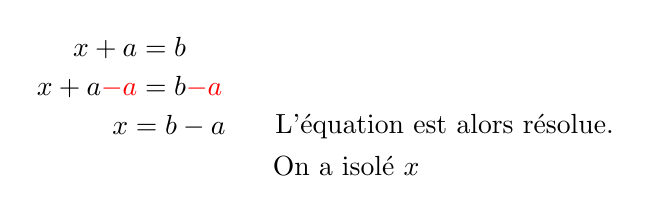
\begin{tikzpicture}
\node at (15, 3) {$ x+a=b$} ; 
\node at (15, 2.5) {$ x + a \textcolor {red} {-a} = b \textcolor {red}{-a}$} ; 
\node at (15.5, 2) {$ x = b-a $} ;  
\node at (19, 2) {L'équation est alors résolue.} ;  
\node at (17.75 , 1.5) {\vocabulaire{On a isolé $x$}} ;  
\end{tikzpicture}    
 
\bigskip 

\Asavoir{{\large 2) }\underline{Équations de la forme $ax=b$}} 

Pour isoler $x$, on multiplie par $\textcolor{red}{\dfrac{1}{a}}$  chaque membre 



\begin{tabular}{M{3.5cm}M{10cm}}
$ ax=b$   & \\
$   \textcolor {red} {\dfrac{1}{\cancel{a}}} \times \cancel{a}x = b \times \textcolor {red}{\dfrac{1}{a}}$   \\
$ x = b-a $   & 
L'équation est alors résolue.  \\
\vocabulaire{On a isolé $x$}  \\ 
\end{tabular}     
   
\bigskip 

\Asavoir{{\large 3) }\underline{Équations de la forme $ax + b = c$}} 

\medskip

Pour isoler $x$, on applique \ding{172}, puis \ding{173}.

\medskip

\newcommand{\xdownarrow}[1]{%
  {\left\downarrow\vbox to #1{}\right.\kern-\nulldelimiterspace}
}

\begin{tabular}{ll}
$ ax + b = c$   & \multirow{2}{5cm}{\methode{ $\Big\downarrow$ On applique \ding{172}} } \\
$  ax + b \textcolor {red} {-b} = c  \textcolor {red} {-b}  $  &   \\
$  ax = c -b $ & \methode{On se retrouve en \ding{173}} \\
$   \textcolor {red} {\dfrac{1}{\cancel{a}}} \times \cancel{a}x = (c - b) \times \textcolor {red} {\dfrac{1}{a}}$  & \methode{$\Big\downarrow$ On applique \ding{173}} \\
$ x = \dfrac{c-b}{a}$   & \multirow{2}{5cm} { L'équation est alors résolue. \\
 \vocabulaire{On a isolé $x$} } \\ 
\end{tabular} 

   
\bigskip 

\Asavoir{{\large 4) }\underline{Équations de la forme $ax + b = cx + d$}} 

\medskip

Pour isoler $x$, on ajoute $\textcolor{red}{-cx}$ à chaque membres et on est alors ramené au cas 
\ding{174}.

\medskip

\begin{tabular}{ll}
$ ax + b = cx +d $   & \multirow{2}{5cm}{\methode{ $\Big\downarrow$ On soustrait \textcolor{red}{cx} }} \\
$ \textcolor{red}{-cx} + ax + b = \textcolor{red}{-cx} + cx +d $   & \\
$  -cx +ax + b \textcolor {red} {-b} = d  \textcolor {red} {-b}  $  &   \\
$  (a - c)x   = d $ & \methode{On se retrouve en \ding{174}} \\
$  (a - c)x   = d  -b $ & \methode{$\big\downarrow$  On applique le cas  \ding{172}} \\
$  x = \dfrac{d-b}{a-c}$  & \methode{$\Big\downarrow$ On applique \ding{173}} \\
\end{tabular} 

 L'équation est alors résolue. \\   \vocabulaire{On a isolé $x$}  \\ 

   
\bigskip 

\Asavoir{{\large 5) }\underline{Équations d'autres formes}}


\medskip


En développant les calculs, et en simplifiant, on pourra toujours, en quatrième, se ramener au cas  \ding{172}, \ding{173}, \ding{174} ou \ding{175}.

\newpage

                 
                 \intitule{Équations du premier degré} 
                 
                 \centerline{\Asavoir{\Large Exemples rédigés de cinq types}}   
                 
\bigskip                  
                 
                 
\Asavoir{{\large 1) }\underline{Équations de la forme $x +a = b$}}   \hspace*{2cm} \vocabulaire{Cas 1}

\bigskip 

\begin{tabular}{lM{3cm}|M{1cm}l}

$x+3 = 0$ & \multirow{2}{3cm}{\methode{$\Big\downarrow$ On ajoute -3} }  & & $x +3 = 7 $\\
$x=-3$   &  & & $x+3 -3 = 7 -3 $\\
  &  & & $x = 4 $\\
$\mathcal{S} =\left\lbrace -3 \right\rbrace$ &  & & $\mathcal{S} =\left\lbrace 4 \right\rbrace$ \\  
  
\end{tabular}
              
\bigskip                  
                 
                 
\Asavoir{{\large 2) }\underline{Équations de la forme $ax = b$}}   \hspace*{2cm} \vocabulaire{Cas 2}

\bigskip 

\begin{tabular}{lM{3.5cm}|M{1cm}l}

$2x = 0$ & \multirow{2}{3cm}{\methode{$\Big\downarrow \mathrm{On\; multiplie\; par\; } \dfrac{1}{2}$} }  & & $2x = 3 $\\
$ \cancel{2}x \textcolor{red}{\times \dfrac{1}{\cancel{2}}}=0$   &  & & $ \cancel{2}x \textcolor{red}{\times \dfrac{1}{\cancel{2}}} = 3 \textcolor{red}{\times \dfrac{1}{2}} $\\
& & & $x = \dfrac{3}{2}$\\
$\mathcal{S} =\left\lbrace 0 \right\rbrace$ &  &  & $\mathcal{S} =\left\lbrace \dfrac{3}{2} \right\rbrace$ \\  
\end{tabular}

\bigskip                  
              
                 
\Asavoir{{\large 3) }\underline{Équations de la forme $ax +b = c$}} 

\bigskip 

\begin{tabular}{lM{4cm}|M{1cm}l}

$4x + 5 = 0$ & 
   \multirow{2}{3cm}{\vocabulaire {$\approx$  \ding{172}} \methode{$\Big\downarrow$ On ajoute -5} }  & & $9x + 6 = - 7 $\\
$4x= -5 $   &  & &$9x + 6 -6   = - 7 -6 $\\
$\cancel{4}x \times \dfrac{1}{\cancel{4}} = - 5 \times \dfrac{1}{4} $  & 
   \multirow{3}{4cm}{\vocabulaire {$\approx$  \ding{173}} \methode{$\Big\downarrow \mathrm{On\; multiplie\; par\; } \dfrac{1}{4}$}}  & & $9x = -13  $\\
 &  & & $ \dfrac{1}{\cancel{9}} \times \cancel{9}x = -13 \times \dfrac{1}{9} $\\   
$x = -\dfrac{5}{4} $   &  & & $x = - \dfrac{13}{9} $\\
 &  & & \\  
$\mathcal{S} =\left\lbrace -\dfrac{5}{4} \right\rbrace$ & \multicolumn{1}{c|}{\methode {Fini}} & &  $\mathcal{S} =\left\lbrace  -\dfrac{13}{9} \right\rbrace$ \\    
\end{tabular}          
  

\bigskip                  
 
             
                 
\Asavoir{{\large 4) }\underline{Équations de la forme $ax +b = cx +d $}} 

\bigskip 

\iffalse 


\makeatletter
\newdimen\multi@col@width
\newdimen\multi@col@margin
\newcount\multi@col@count
\multi@col@width=0pt
\tikzset{
  multicol/.code={%
    \global\multi@col@count=#1\relax
    \global\let\orig@pgfmatrixendcode=\pgfmatrixendcode
    \global\let\orig@pgfmatrixemptycode=\pgfmatrixemptycode
    \def\pgfmatrixendcode##1{\orig@pgfmatrixendcode%
      ##1%
      \pgfutil@tempdima=\pgf@picmaxx
      \global\multi@col@margin=\pgf@picminx
      \advance\pgfutil@tempdima by -\pgf@picminx
      \divide\pgfutil@tempdima by #1\relax
      \global\multi@col@width=\pgfutil@tempdima
      \pgf@picmaxx=.5\multi@col@width
      \pgf@picminx=-.5\multi@col@width
      \global\pgf@picmaxx=\pgf@picmaxx
      \global\pgf@picminx=\pgf@picminx
      \gdef\multi@adjust@position{%
        \setbox\pgf@matrix@cell=\hbox\bgroup
        \hfil\hskip-\multi@col@margin
        \hfil\hskip-.5\multi@col@width
        \box\pgf@matrix@cell
        \egroup
      }%
      \gdef\multi@temp{\aftergroup\multi@adjust@position}%
      \aftergroup\multi@temp
    }
    \gdef\pgfmatrixemptycode{%
      \orig@pgfmatrixemptycode
      \global\advance\multi@col@count by -1\relax
      \global\pgf@picmaxx=.5\multi@col@width
      \global\pgf@picminx=-.5\multi@col@width
      \ifnum\multi@col@count=1\relax
       \global\let\pgfmatrixemptycode=\orig@pgfmatrixemptycode
      \fi
    }
  }
}
\makeatother

\fi

\setbox1=\vtop{ \hsize=5cm \null % null assure l'alignement par le haut 
\begin{tikzpicture}% [every node/.style={anchor=west}]
  \matrix (m) [matrix of math nodes,
row sep=0cm,column sep=0cm,  
% nodes={rectangle, draw},  
%    nodes in empty cells,
column 1/.style={anchor=base east},
column 3/.style={anchor=base west}]{
3x -5                                         &=& x + 1  \\%  
3x \; \TextSoulign{blue}{-x} -5               &=& x +1 \;\TextSoulign{blue}{-x} \\
2x -5                                         &=& |(a)| 1  \vocabulaire{\hspace{1.5cm}\text{\ding{174}}} \\
2x -5 \; \TextSoulign{blue}{+5}               &=& |(b)|1+\;\TextSoulign{blue}{5}       \\
2x                                            &=& 6 \vocabulaire{\hspace{1.5cm}\text{\ding{173}}} \\
2x \; \TextSoulign{blue}{\times \dfrac{1}{2}} &=& 6 \;\TextSoulign{blue}{\times \dfrac{1}{2}}  \\
x                                             &=& 3 \\
 \hbox to .1cm{}                              & &   \\
\textcolor{white}{\mathcal{S} = \left\lbrace -\dfrac{5}{4} \right\rbrace}& & \hbox to .1cm{}\\
}; 
\draw[color=blue,->,>=latex] (a) to[out=0,in=0]node[midway,below]
{\vocabulaire {\ding{172}}}   (b);       
\node[fit=(m-9-1)(m-9-3)]{$\mathcal{S} = \left\lbrace 3 \right\rbrace$};      
\end{tikzpicture}}

\setbox2=\vtop { \hsize=5cm  \null
\begin{tikzpicture}% [every node/.style={anchor=west}]
  \matrix (n) [matrix of math nodes,
row sep=0cm,column sep=0cm,  
% nodes={rectangle, draw},  
%    nodes in empty cells,
column 1/.style={anchor=base east},
column 3/.style={anchor=base west}]{
|(c)|   3x -5    &=& |(d)|  9x +1 \\
 \hbox to .1cm{} & &   \\               
|(e)| 3x -9x     &=& |(f)| 1 + 5    \\
 -6x &=& |(g)| 6 \\   
x &=& |(h)| \dfrac{6}{-6} \\   
x &=& -1  \\
 \hbox to .1cm{}                              & &   \\
\textcolor{white}{\mathcal{S} = \left\lbrace -1 \right\rbrace}& & \hbox to .1cm{} & \\
 }; 
\draw[color=blue,->,>=latex] (c) to[out=-30,in=110]node[midway,right] {} (f) ;   
\draw[color=blue,->,>=latex] (d) to[out=190,in=north east]node[midway,right] {} (e) ;  
\draw[color=blue,->,>=latex] (g) to[out=0,in=0]node[midway,right] {\methode{On divise par -6}} (h) ;    
\node[fit=(n-8-1)(n-8-3)]{$\mathcal{S} = \left\lbrace -1 \right\rbrace$};         
\end{tikzpicture}}


\centerline{ \box1 \quad\vrule\quad \box2 \hfill}

\newpage

\Asavoir{{\large 5) }\underline{Plus dur ...}} 

\medskip 

\begin{tikzpicture}% [every node/.style={anchor=west}]
  \matrix (m) [matrix of math nodes,
row sep=0cm,column sep=0cm,  
% nodes={rectangle, draw},  
%    nodes in empty cells,
column 2/.style={anchor=base east},
column 4/.style={anchor=base west}
]{
\Asavoir{\large a) } & 6 \textcolor{blue}{\underbrace{\textcolor{black}{-4 (1-x)}}} &=& |(a)| 3x + 5 \\
   & 6  -4 \times 1 - 4\times (-x) &=& |(b)| 3x + 5  \\
   & 6  -4  + 4x &=&  3x + 5  \\   
   & 2  + 4x &=&  3x + 5  \\   
   & 2  + 4x -3x &=& 3x + 5 -3x  \\   
   & 2 + x      &=& 5 \\
   & 2  + x -2 &=& 5 -2 \\     
   & x &=& 3 \\  
 \hbox to .1cm{}                              & &   \\   
   & & & \hspace*{1cm}\mathcal{S} =\left\lbrace 3 \right\rbrace \\        
}; 
\node [right = 1cm of a.west] (c) {} ; 
\node [right = 1cm of b.west] (d) {} ; 
\draw[color=blue,->,>=latex] (c) to[out=0,in=0] node[midway,right] {\hspace*{.5cm} \parbox{3cm}{Ne ressemble pas à\\ un cas connu ...\\
On développe }}  (d) ; 
\end{tikzpicture}


\bigskip 

\begin{tikzpicture}% [every node/.style={anchor=west}]
  \matrix (m) [matrix of math nodes,
row sep=0cm,column sep=0cm,  
% nodes={rectangle, draw},  
%    nodes in empty cells,
column 2/.style={anchor=base east},
column 4/.style={anchor=base west}
]{
\Asavoir{\large b) } 
   & 3 - \big[5 -(x-7)\big] &=& |(a)| 2(x-4)-1 \\
   & 3 - (5 -x +7)          &=& |(b)| 2x-2\times 4 -1 \\
   &3 -5 +x -7              &=&  2x -8 -1 \\     
   & x - 9                  &=& |(c)| 2x - 9   \\   
   & x                      &=& |(d)| 2x \\     
   & x                      &=& |(i)| 0 \\  
 \hbox to .1cm{}                              & &   \\    
   & & & \hspace*{1.5cm}\mathcal{S} =\left\lbrace 0 \right\rbrace \\         
}; 
\node [right = 2cm of a.west] (e) {} ; 
\node [right = 1cm of b.west] (f) {} ; 
\draw[color=blue,->,>=latex] (e) to[out=0,in=0] node[midway,right]{\hspace*{.5cm} On développe ...} (b); \\ 
\node [right = 1.5cm of c.west] (g) {} ; 
\node [right = 1.25cm of d.west] (h) {} ; 
\draw[color=blue,->,>=latex] (g) to[out=0,in=0] node[midway,right]{\hspace*{.5cm} On soustrait 9} (h); \\ 
\node [right = 1cm of d.west] (k) {} ; 
\node [right = 1cm of i.west] (j) {} ; 
\draw[color=blue,->,>=latex] (k) to[out=0,in=0] node[midway,right]{\hspace*{.5cm} On soustrait $x$ à gauche et à droite} (j); \\ 
\end{tikzpicture} 

\newpage 


\ifdefined\COMPLETE
\else
    \end{document}
\fi \newpage

\ifdefined\COMPLETE
\else
    \input{./preambule-sacha-utf8.ltx}
    \begin{document}
\fi

                 
                 \intitule{Inéquations du premier degré : cours} 
                 
\bigskip     

De manière générale :

\begin{itemize}
\item Une inéquation se résout comme une équation : 
     \begin{itemize}
     \item [$\hookrightarrow$] le but est toujours d'isoler $x$ ; 
     \item [$\hookrightarrow$] les formes sont les mêmes.
     \end{itemize}
\item Le $=$ devient $<$, $>$, $\leqslant$, $\geqslant$.     
\end{itemize}    

\bigskip 

\Asavoir{Une règle supplémentaire}     


\medskip 

Si on \Asavoir{multiplie} par un nombre \TextSoulign{red}{négatif}, on change le signe de l'inéquation (\vocabulaire{le sens}).
   

\medskip 

\begin{description}
\item $<$ devient $>$
\item $>$ devient $<$
\item $\leqslant$ devient $\geqslant$
\item $\geqslant$ devient $\leqslant$
\end{description}             

\bigskip         
%                 \intitule{Inéquations du premier degré} 
                 
                 \centerline{\intitule{Exemples rédigés...}}   
                 
\bigskip   

On rédigera ici 2 exemples, pour montrer le changement de sens lorsque l'on multiplie par un nombre négatif.

Pour la technique de résolution, consulter les exemples rédigés de la fiche sur les équations.

\setbox1=\vtop{ \hsize=5cm \null % null assure l'alignement par le haut 
\begin{tikzpicture}% [every node/.style={anchor=west}]
  \matrix (m) [matrix of math nodes,
row sep=0cm,column sep=0cm,  
]{
2x -5            &\leqslant& |(a)| 0  \\%  
2x               &\leqslant& |(b)|5 \\
x                &\leqslant& |(c)| \dfrac{5}{2} \\
};  
% \node [right = 1cm of a.west] (k) {} ; 
% \node [right = 1cm of i.west] (j) {} ; 
\draw[color=blue,->,>=latex] (a) to[out=0,in=0] node[midway,right]{ On ajoute 5} (b); 
\draw[color=blue,->,>=latex] (b) to[out=0,in=0] node[midway,right]{ On divise par 2} (c);
\end{tikzpicture}

\vocabulaire{$2>0$, donc pas de changement de sens}}

\setbox2=\vtop { \hsize=5cm  \null
\begin{tikzpicture}% [every node/.style={anchor=west}]
  \matrix (m) [matrix of math nodes,
row sep=0cm,column sep=0cm,  
]{
-3x +7           &\leqslant& |(a)| 0  \\%  
-3x               &\leqslant& |(b)| -7\\
x                &\textcolor{red}{\geqslant}& |(c)| \dfrac{-7}{-3} \\
x                &\geqslant& |(d)| \dfrac{7}{3} \\
};  
% \node [right = 1cm of a.west] (k) {} ; 
% \node [right = 1cm of i.west] (j) {} ; 
\draw[color=blue,->,>=latex] (a) to[out=0,in=0] node[midway,right]{ On ajoute -7} (b); 
\draw[color=blue,->,>=latex] (b) to[out=0,in=0] node[midway,right]{ On divise par -3} (c);
\draw[color=blue,->,>=latex] (c) to[out=0,in=0] node[midway,right]{ On simplifie} (d);
\end{tikzpicture}
\vocabulaire{$-3<0$, donc changement de sens}}  


\centerline{ \box1 \quad\vrule\quad \box2 \hfill}



\ifdefined\COMPLETE
\else
    \end{document}
\fi \newpage

\ifdefined\COMPLETE
\else
    \input{./preambule-sacha-utf8.ltx}
    \begin{document}
\fi

                 \intitule{Puissance : cours} 
                 
\bigskip   

\Asavoir{Définition } : Élever un nombre à la puissance $n$, c'est multiplier ce nombre $n$ fois par lui-même.

\medskip 

\underline{Exemple :} $10^3 = 10 \times 10 \times 10 = 1 000$

\medskip 

\vocabulaire {Remarque : } Si $n$ est négatif, on passe à l'inverse.

\medskip 

\underline{Exemple :} $10^{-4} = \dfrac{1}{10^4} = \dfrac{1}{10 \times 10 \times 10 \times 10} = \dfrac{1}{10 000}$ 

\medskip 

\vocabulaire {Remarque : } Tout nombre élevé à la puissance $0$ vaut $1$.

\bigskip   

\Asavoir{Règle de calcul}

\medskip 

\begin{tabular}{rr@{$\;\;$}c@{$\;\;$}ll}
$\bullet$ & $a^m \times a^n $   & $=$ & $ a^{m+n}$ &  {\vocabulaire {($\times$ devient $+$)}}  \\  
$\bullet$ & $\dfrac{a^m}{a^n}$  & $=$ & $a^{m-n}$  &  {\vocabulaire {($\div$ devient $-$)}} \\   
$\bullet$ & $\big( a^m\big)^n$  & $=$ & 
                       $a^{m\times n}$ & {\vocabulaire {(puissance devient $\times$)}} \\ 
$\bullet$ & $a^m \times b^m$    & $=$ & $\big(a\times b\big)^m$ & \multirow{2}{*}{\textcolor{darkgreen}{
                      $ \left\rbrace 
                         \begin{array}{l}
                          \\ \text {(Réunion de même puissace)} \\ \\
                          \end{array}  
                          \right. $ 
} }    \\
$\bullet$ & $ \dfrac{a^m}{b^m}$ & $=$ & $\left(\dfrac{a}{b}\right)^m$ &                                        
\end{tabular}


%---------
\bigskip         
%                 \intitule{Puissance} 
                 
                 \centerline{\intitule{\ Quelques exemples rédigés}} 

\bigskip                   

\setbox1=\vtop{ \hsize=5cm \null % null assure l'alignement par le haut 
\begin{tikzpicture}% [every node/.style={anchor=west}]
  \matrix (m) [matrix of math nodes,
row sep=0cm,column sep=0cm, 
column 1/.style={anchor=base east},
column 3/.style={anchor=base west} 
]{
A      &=&  (-2)^4 \\
       &=&  (-2)\times (-2)\times (-2)\times (-2) \\
       &=&  16  \\
};  
\end{tikzpicture}}

\setbox2=\vtop { \hsize=5cm  \null
\begin{tikzpicture}% [every node/.style={anchor=west}]
  \matrix (m) [matrix of math nodes,
row sep=0cm,column sep=0cm,
column 1/.style={anchor=base east},
column 3/.style={anchor=base west}  
]{
B      &=& |(a)|       4^{-3} \\
       &=& |(b)| \dfrac{1}{4^3} \\
       &=& |(c)|\dfrac{1}{4\times 4\times 4} \\
       &=& \dfrac{1}{64} \\
};  
\node [right = 1cm of a.west] (d) {} ; 
\node [right = .5cm of b.west] (e) {} ; 
\node [right = 1cm of b.west] (g) {} ; 
\node [right = 1.5cm of c.west] (f) {} ; 
\draw[color=blue,->,>=latex] (d) to[out=0,in=0] node[midway,right] {\hspace*{.5cm} \parbox{5cm}{
$n$ est négatif donc \\ on passe à l'inverse.
}}  (e) ; 
\draw[color=blue,->,>=latex] (g) to[out=0,in=0] node[midway,right] {\hspace*{.5cm} \parbox{5cm}{
On revient à la définition.
}}  (f) ; 
\end{tikzpicture}}  


\centerline{ \box1 \quad\vrule\quad \box2 \hfill}    

\medskip 
\hrulefill
\medskip 
\setbox1=\vtop{ \hsize=7.5cm \null % null assure l'alignement par le haut 
\begin{tikzpicture}% [every node/.style={anchor=west}]
  \matrix (m) [matrix of math nodes,
row sep=0cm,column sep=0cm, 
column 1/.style={anchor=base east},
column 3/.style={anchor=base west},
column 4/.style={anchor=base west} 
]{
C      &=&  |(a)| \textcolor{blue}{\underbrace{\textcolor{black}{2^2}}}  
               \times (2 \textcolor{blue}{\underbrace{\textcolor{black}{+3^3}}}          
               )- \textcolor{blue}{\underbrace{\textcolor{black}{5^0}}}  
                                                          &  \text{\methode{Puissance d'abord}} \\
       &=& |(b)| \;\; 4  \;\;\times \;\; ( \textcolor{blue}{\underbrace{\textcolor{black}{2+27}}} ) \;\; -1 
                                                          &  \text{\methode{Puis parenthèses}} \\
       &=& |(c)| \textcolor{blue}{\underbrace{\textcolor{black}{ 4 \quad \; \times \quad 29}}} \quad  -1 
                                                          &  \text{\methode{Puis produit}} \\
       &=& \quad  116 \quad  -1 \\ 
       &=&  115 \\               
};  
\end{tikzpicture}}

\setbox2=\vtop { \hsize=5cm  \null
\begin{tikzpicture}% [every node/.style={anchor=west}]
  \matrix (m) [matrix of math nodes,
row sep=0cm,column sep=0cm,
column 1/.style={anchor=base east},
column 3/.style={anchor=base west}  
]{
D  &=& |(a)|   \dfrac{5^{-1}}{1^{-4}}  \\
   &=& |(b)|  \displaystyle{\;\;\dfrac{1}{5^1}\;\; \over \;\;\dfrac{1}{1^{4}}\;\;} \\
   &=& |(c)|  \dfrac{1}{5} \times 1^4\\
   &=& \dfrac{1}{5} \\
};  
\node [right = 1cm of a.west] (d) {} ; 
\node [right = .5cm of b.west] (e) {} ; 
\node [right = 1cm of b.west] (g) {} ; 
\node [right = 1cm of c.west] (f) {} ; 
\draw[color=blue,->,>=latex] (d) to[out=0,in=0] node[midway,right] {\hspace*{.5cm} \parbox{5cm}{On passe à l'inverse deux fois }}  (e) ; 
\draw[color=blue,->,>=latex] (g) to[out=0,in=0] node[midway,right] {\hspace*{.5cm} \parbox{5cm}{Diviser revient à multiplier par l'inverse}}  (f) ; 
\end{tikzpicture}

\methode{Quelque soit $n$, $1^n = 1$}}  


\centerline{ \box1 \quad\vrule\quad \box2 \hfill}    
  
\newpage 

\begin{tikzpicture}% [every node/.style={anchor=west}]
  \matrix (m) [matrix of math nodes,
row sep=0cm,column sep=0cm, 
column 1/.style={anchor=base east},
column 3/.style={anchor=base west},
column 4/.style={anchor=base west} 
]{
E      &=& |(a)|  2^2 \times 3^3 \times 2^3 \times 3^{-3}\\
       &=& |(b)| \textcolor{blue}{\underbrace{\textcolor{black}{ 2^2 \times 2^3}}}
         \times  \textcolor{blue}{\underbrace{\textcolor{black}{ 3^3 \times 3^{-3}}}} \\\\
       &=& |(c)| \quad 2^5 \quad \times \quad  \; 3^0 \\
       &=& |(d)| 2^5 \times 1\\ 
       &=&   32 \\               
};  
\node [right = 2.75cm of a.west] (e) {} ; 
\node [right = 2.6cm of b.west] (f) {} ; 
\node [right = 2.4cm of b.west] (g) {} ; 
\node [right = 2.5cm of c.west] (h) {} ; 
\node [right = 2.3cm of c.west] (i) {} ; 
\node [right = 2cm of d.west] (j) {} ; 
\draw[color=blue,->,>=latex] (e) to[out=0,in=0] node[midway,right] {\hspace*{.5cm} \parbox{5cm}{
On regroupe
}}  (f) ; 
\draw[color=blue,->,>=latex] (g) to[out=0,in=0] node[midway,right] {\hspace*{.5cm} \parbox{5cm}{
On simplifie ($\times$ devient $+$)
}}  (h) ; 
\draw[color=blue,->,>=latex] (i) to[out=0,in=0] node[midway,right] {\hspace*{.25cm} \parbox{5cm}{
On simplifie ($\times$ devient $+$)
}}  (j) ; 
\end{tikzpicture}

\bigskip 

\begin{tikzpicture}% [every node/.style={anchor=west}]
  \matrix (m) [matrix of math nodes,
row sep=0cm,column sep=0cm, 
column 1/.style={anchor=base east},
column 3/.style={anchor=base west},
column 4/.style={anchor=base west} 
]{
F      &=& |(a)| \dfrac{3^{-6} \times 3^2 \times 3^{-4}}{3^{-8} \times 3^{-2}}\\
       &=& |(b)| \dfrac{3^{-6+2-4}}{3^{-8-2}}\\
       &=& |(c)| \dfrac{3^{-8}}{3^{-10}}\\
       &=& |(d)| 3^{-8-(-10)} \\ 
       &=&       3^2   \\   
       &=& 9      \\      
};  
\node [right = 2.75cm of a.west] (e) {} ; 
\node [right = 2.6cm of b.west] (f) {} ; 
\node [right = 2.4cm of b.west] (g) {} ; 
\node [right = 2.5cm of c.west] (h) {} ; 
\node [right = 2.3cm of c.west] (i) {} ; 
\node [right = 2cm of d.west] (j) {} ; 
\draw[=bluecolor,->,>=latex] (e) to[out=0,in=0] node[midway,right] {\hspace*{.5cm} \parbox{5cm}{
$\times$ devient $+$ au numérateur et au dénominateur
}}  (f) ; 
\draw[color=blue,->,>=latex] (g) to[out=0,in=0] node[midway,right] {\hspace*{.5cm} \parbox{5cm}{
On calcule l'exposant
}}  (h) ; 
\draw[color=blue,->,>=latex] (i) to[out=0,in=0] node[midway,right] {\hspace*{.25cm} \parbox{5cm}{
$\div$ devient $-$}}   (j) ;  
\end{tikzpicture}     

\newpage



\ifdefined\COMPLETE
\else
    \end{document}
\fi \newpage

\ifdefined\COMPLETE
\else
    \input{./preambule-2010-utf8.ltx}
    \usepackage{frcursive}
    \usepackage{calligra}
    \begin{document}
\fi

\iffalse

\begin{tikzpicture}[line cap=round,line join=round,>=triangle 45,x=10mm,y=10mm,scale=1]
\begin{tiny}
    \tkzDefPoint[label=below left:A](0,0){A}
    \tkzDefPoint [label=below right:B](1.5,0){B}
    \tkzDefPoint[label=above:C](0,2){C}
\draw [black,fill=yellow!20] (A) --  (B) -- (C) -- cycle  ;
\tkzMarkAngle[color=red, size=.6](C,B,A)
\tkzLabelAngle[pos=.8,color=red,font=\tiny](A,B,C){40\textdegree}
\tkzMarkRightAngle[color=red](C,A,B)
\tkzLabelSegments[color=red,below=4pt](A,B){$3cm$}
\end{tiny}
\end{tikzpicture}
\fi

\begin{alterqcm}[lq=11cm]
\AQquestion[br=2]{\setbox2=\hbox{\begin{minipage}[t]{5cm}
                            Dans la situation ci-contre, \\
                            pour calculer $AC$, on utilise\ldots
                                 \end{minipage}}                           
                   \setbox3=\hbox{\begin{minipage}[b]{5cm}
\begin{tikzpicture}[scale=.5,rotate=-15]
\tkzDefPoint(0,0){A}
\tkzDefShiftPoint[A](0:2.2){M}
\tkzDefShiftPoint[A](30:3){N}
\tkzDefShiftPoint[A](0:6){B}
\tkzDefShiftPoint[A](30:8){C}
\tkzDrawSegments(A,B B,C C,A M,N)
\tkzDrawPoints(A,B,C,M,N)
\tkzLabelPoints[left](A) \tkzLabelPoints[below](B) \tkzLabelPoints[right](C)
\tkzLabelPoints[below](M) \tkzLabelPoints[above](N)
\tkzLabelSegment[below,pos=.5,red](A,M){2}
\tkzLabelSegment[below,pos=.5,red](M,B){4}
\tkzLabelSegment[above,pos=.5,red](A,N){5}
\end{tikzpicture}
                                 \end{minipage}
                                  }   
\begin{tabular}{b{5cm}p{5cm}}
\raisebox{25mm}{\box2} & {\box3}\\
\end{tabular}
}{%
 {$\cos(\widehat{B})$},
 {$\sin(\widehat{B})$}, 
 {$\tan(\widehat{B})$}
} 
\AQquestion[br=2]{\setbox2=\hbox{\begin{minipage}[t]{5cm}
                            Dans la situation ci-contre, \\
                            le théorême de {\sc Thalès} permet d'écrire\ldots
                                 \end{minipage}}                           
                   \setbox3=\hbox{\begin{minipage}[b]{5cm}
\begin{tikzpicture}[scale=.4,rotate=-50]
\tkzDefPoint(0,0){O}
\tkzDefShiftPoint[O](0:-2.2){A}
\tkzDefShiftPoint[O](30:-3){B}
\tkzDefShiftPoint[O](0:6){D}
\tkzDefShiftPoint[O](30:8){C}
\tkzDrawSegments(A,B B,C A,D D,C)
\tkzDrawPoints(A,B,C,D,O)
\tkzLabelPoints[above right](O) \tkzLabelPoints[left](B) \tkzLabelPoints[right](C)
\tkzLabelPoints[below](D) \tkzLabelPoints[above](A)
%\tkzLabelSegment[below,pos=.5,red](A,M){2}
%\tkzLabelSegment[below,pos=.5,red](M,B){4}
%\tkzLabelSegment[above,pos=.5,red](A,N){5}
\end{tikzpicture}
                                 \end{minipage}
                                  }   
\begin{tabular}{p{5cm}b{5cm}}
 {\box3} & \raisebox{25mm}{\box2} \\
\end{tabular}
}{%
 {$\dfrac{OA}{OB} = \dfrac{OD}{OC} = \dfrac{AB}{CD}$},
 {$\dfrac{OA}{OC} = \dfrac{OB}{OD} = \dfrac{AB}{CD}$}, 
 {$\dfrac{OA}{OD} = \dfrac{OB}{OC} = \dfrac{AB}{CD}$}
} 

\AQquestion[br=2]{\setbox2=\hbox{\begin{minipage}[t]{6.5cm}
                           Avec les données de la figure à main levée ci-contre, 
                           on peut affirmer que la longueur de $FM$ est égale à\ldots
                                 \end{minipage}}                           
                   \setbox3=\hbox{\begin{minipage}[b]{3cm}
\font\pc=cmitt10 \rm
\begin{tikzpicture}[scale=.4,rotate=10,decoration={random   steps, amplitude=1pt,segment  length=3pt}]
\begin{tiny}
\tkzDefPoint(0,0){A}
\tkzDefShiftPoint[A](0:-2.2){N}
\tkzDefShiftPoint[A](40:-3){E}
\tkzDefShiftPoint[A](40:5){F}
\tkzDefShiftPoint[A](0:5){M}
\draw[decorate,decoration=random steps,segment length=4.5mm] (E) -- (F) -- (M) -- (N) -- cycle ; 
\tkzDrawPoints(A,E,F, M,N)
%\tkzLabelPoints[above left](A) \tkzLabelPoints[below right ](E) \tkzLabelPoints[above right](F)
%\tkzLabelPoints[above](N) \tkzLabelPoints[right](M)
\draw (A) [above left] node  {\pc A} ;
\draw (E) [below right ] node  {\pc E} ;
\draw (F) [above right] node  {\pc F} ;
\draw (M) [right] node  {\pc M} ;
\draw (N) [above] node  {\pc N} ;
\tkzLabelSegment[below right,pos=.5,red](A,E){\pc 3}
\tkzLabelSegment[left,pos=.5,red](E,N){\pc  2}
\tkzLabelSegment[above left ,pos=.5,red](A,F){\pc  5}
\draw (2,-1.5) node []{ { {\pc (FM)//(EN)}}};
\end{tiny}
\end{tikzpicture}
\end{minipage}
                                  }   
\begin{tabular}{p{3.5cm}b{7cm}}
 {\box3} & \raisebox{25mm}{\box2} \\
\end{tabular}
}{%
 {3,3},
 {$\dfrac{10}{3}$}, 
 {4}
} 


 \AQquestion[br=2]{$ABC$ est un triangle tel que $AB=3cm$ et $AC=4cm$.\\
 $M$ est un point de $(AB)$ et $N$, un point de $(AC)$, tel que : 
 $AM=1,5cm$ et $AN=2cm$\\
 Pour pouvoir en déduire que : $(MN)/sslash (BC)$, il faut savoir aussi que\ldots}
  {%
   {\begin{minipage}[t]{6cm} $A,M,B \; \mathrm{ et } \;  A, N, C$ \\ sont dans le même ordre\end{minipage}},
   {\begin{minipage}[t]{6cm}  $A,M,B \; \mathrm{ et } \; A, C, N$ \\ sont dans le même ordre
    \end{minipage}},
   {\begin{minipage}[t]{6cm}  $A,N,B \; \mathrm{ et } \; A, M, C$ \\ sont dans le même ordre
    \end{minipage}}
 }
 
 \AQquestion[br=2]{Avec les données ci-dessous\ldots\\
\begin{tikzpicture}[scale=.5]
\tkzDefPoint(0,0){A}
\tkzDefShiftPoint[A](0:4){B}
\tkzDefShiftPoint[A](90:3){C}
\tkzDefShiftPoint[A](0:6){M}
\tkzDefShiftPoint[A](90:5){N}
\tkzDrawSegments(A,N A,M  C,B M,N)
%\tkzDrawPoints(A,B,C,M,N)
\tkzLabelPoints[below left](A) \tkzLabelPoints[below](B) \tkzLabelPoints[left ](C)
\tkzLabelPoints[below](M) \tkzLabelPoints[below left](N)
\tkzLabelSegment[left,pos=.5,red](A,C){3}
\tkzLabelSegment[below,pos=.5,red](A,B){4}
\tkzLabelSegment[below,pos=.5,red](B,M){1}
\end{tikzpicture}
 }
  {%
   {\begin{minipage}[t]{6cm} on calcule $BC$ avec le théorème de {\sc Pythagore}, \end{minipage}},
   {\begin{minipage}[t]{6cm} on calcule $BC$ avec le théorème de {\sc Thalès} 
    \end{minipage}},
   {\begin{minipage}[t]{6cm} on ne peut pas calculer $BC$
    \end{minipage}}
 }

\end{alterqcm}


\ifdefined\COMPLETE
\else
    \end{document}
\fi \newpage

\ifdefined\COMPLETE
\else
    \input{./preambule-sacha-utf8.ltx}
    \begin{document}
\fi

             
                 \intitule{Droite des milieux : cours } 

\Asavoir{{\large I)} Théorème de parallélisme}

\setbox1=\vtop { \hsize=5cm  \null
\begin{tikzpicture}[line cap=round,line join=round,>=triangle 45,x=1.0cm,y=1.0cm,scale=.6, rotate=0]
\begin{scriptsize}
% \draw (0.,0.) node [above ] {$A$} -- (2.18,1.) node [right] {$M$} ; 
\draw   (0,0) node [below] {$B$} -- node[midway,rotate=50] {$\vert\vert$}
        (3,2) node [left]  {$M$} -- node[midway,rotate=50] {$\vert\vert$} 
        (6,4) node [above] {$A$} -- node[midway,rotate=-20] {\textcolor{red}{ $-$}}
        (5,2) node [right] {$N$} -- node[midway,rotate=-20] {\textcolor{red}{ $-$}}
        (4,0) node [below] {$C$} -- cycle ; 
\draw (3,2) -- (5,2) ;         
\end{scriptsize}        
\end{tikzpicture} }


\begin{tabular}{M{10cm}M{10cm}}
\parbox{10cm}{
   Dans un triangle, si \TextSoulign {blue} {une droite passe par les milieux de deux côtés}, alors elle est parallèle au troisième.
}
 & \box1 
\end{tabular} 

\methode{On utilise ce théorème pour montrer que \underline{deux droites sont parallèles}}

\bigskip 

\Asavoir{{\large II)} Théorème du milieu}

\setbox1=\vtop { \hsize=5cm  \null
\begin{tikzpicture}[line cap=round,line join=round,>=triangle 45,x=1.0cm,y=1.0cm,scale=.6, rotate=0]
\begin{scriptsize}
% \draw (0.,0.) node [above ] {$A$} -- (2.18,1.) node [right] {$M$} ; 
\draw   (0,0) node [below] {$B$} -- node[midway,rotate=50] {\textcolor{red}{$\vert\vert$}}
        (3,2) node [left]  {$M$} -- node[midway,rotate=50] {\textcolor{red}{$\vert\vert$}}
        (6,4) node [above] {$A$} -- 
        (5,2) node [right] {$N$} -- 
        (4,0) node [below] {$C$} -- cycle ; 
\draw (3,2) -- (5,2) ;         
\end{scriptsize}        
\end{tikzpicture} }


\begin{tabular}{M{10cm}M{10cm}}
\parbox{10cm}{
   Dans un triangle, si \TextSoulign {blue} {une droite passe par le milieu d'un côté}, 
   et est \TextSoulign {blue} {parallèle à un second côté}, 
   alors elle coupe le troisième côté en son milieu.
}
 & \box1 
\end{tabular} 

\methode{On utilise ce théorème pour montrer qu'un point est \underline{le milieu d'un segment}}.


\bigskip 

\Asavoir{{\large II)} Théorème des longueurs}

\setbox1=\vtop { \hsize=5cm  \null
\begin{tikzpicture}[line cap=round,line join=round,>=triangle 45,x=1.0cm,y=1.0cm,scale=.6, rotate=0]
\begin{scriptsize}
% \draw (0.,0.) node [above ] {$A$} -- (2.18,1.) node [right] {$M$} ; 
\draw   (0,0) node [below] {$B$} -- node[midway,rotate=50] {$\vert\vert$}
        (3,2) node [left]  {$M$} -- node[midway,rotate=50]  {$\vert\vert$}
        (6,4) node [above] {$A$} -- node[midway,rotate=-20]  {$-$}
        (5,2) node [right] {$N$} -- node[midway,rotate=-20]  {$-$}
        (4,0) node [below] {$C$} -- node[midway,below]  {$4$ cm} cycle ; 
\draw (3,2) -- (5,2) node[midway,below]  {$2$ cm} ;         
\end{scriptsize}        
\end{tikzpicture} }


\begin{tabular}{M{10cm}M{10cm}}
\parbox{10cm}{
   Dans un triangle, la \TextSoulign {blue} {longueur du segment joignant les milieux} de deux côtés est  
   \TextSoulign {blue} {égale à la moitié de celle du troisième côté}. 
 
}
 & \box1 
\end{tabular} 

\methode{On utilise ce théorème pour \underline{calculer une longueur}}.


\newpage        
 %                 \intitule{Droite des milieux} 
                 
                 \centerline{\intitule{Deux exemples rédigés}} 
\setbox1=\vtop { \hsize=5cm  \null
\begin{tikzpicture}[line cap=round,line join=round,>=triangle 45,x=1.0cm,y=1.0cm,scale=.7, rotate=150]
\begin{scriptsize}
\draw   (0,0) node [below] {$C$} -- node[midway,rotate=50] {$\vert\vert$}
        (1.5,2) node [below ] {$F$} -- node[midway,rotate=50]  {$\vert\vert$}
        (3,4) node [below] {$B$} -- node[midway,rotate=-0]  {$-$}
        (4,2) node [below left] {$E$} -- node[midway,rotate=-0]  {$-$}
        (5,0) node [above] {$A$} --  cycle ; 
\draw (.5,2) -- (5,2)  ;  
\draw   (2,0) node [above right] {$D$} --  (3,4)   ;    
\draw (2.5, 2) node   [above] {$G$}  ;      
\end{scriptsize}        
\end{tikzpicture} }                 
                 

\begin{tabular}{M{9cm}M{9cm}}
\parbox{10cm}{
\underline{Exemple 1 : Parallèle et milieu}\\
\\
Soit $ABC$ un triangle et $D$ un point du segment $[AC]$. \\
Soient $E$ et $F$ les \TextSoulign{blue}{milieux} respectifs de $[AB]$ et $[BC]$. \\
Soit $G$ le point d'intersection de $(EF)$ et $(BD)$.  
}
 & \box1 
\end{tabular} 

\underline{a) Démontrer que $(EF)$ et $(AC)$ sont parallèles}

\medskip 

On se place dans le triangle $ABC$.

\addtokomafont{labelinglabel}{\textnormal}

\begin{labeling}{On sait que } 
\item [On sait que ] $[AB)$ et $[BC)$ sont \TextSoulign{blue}{deux demi-droites} d'origine $B$,\\
           les points $B, E$ et $A$ et $B, F$ et $C$ sont  \TextSoulign{blue}{alignés dans cet ordre}, \\
            et que $E$ et $F$ sont les \TextSoulign{blue}{milieux} de $[AB]$ et $[BC]$. 
\item [Or, ] si, dans un triangle, une droite passe par les milieux  de deux côtés, alors elle est parallèle au troisième. 
\item [Donc] $(EF)$ et $(AC$) sont parallèles.             
\end{labeling}

\bigskip 

\underline{b) Démontrer que $G$ est le milieu de $[BD]$}

\begin{labeling}{On sait que } 
\item [On sait que ]  $(EF)$ est \TextSoulign{blue}{parallèle} à $(AC)$, \\
                      $G$ est un point de $[EF]$ et $D$ appartient à $[AC]$.\\
\item [Ainsi] $(FG)$ est parallèle à $(CD)$.            
\end{labeling}

On se place dans le triangle $BCD$.

\begin{labeling}{On sait que } 
\item [On sait que ] $[BC)$ et $[BD)$ sont \TextSoulign{blue}{deux demi-droites} d'origine $B$,\\ 
           les points $B, G, D$ et $B, F, C$ sont  \TextSoulign{blue}{alignés dans cet ordre},\\
$(FG)$ est \TextSoulign{blue}{parallèle} $(CD)$ et que $F$ est le \TextSoulign{blue}{milieu} de $[BC]$, 
\item [Or, ] si, dans un triangle, une droite passe par le milieu d'un côté, 
   et est parallèle à un second côté, alors elle coupe le troisième côté en son milieu.
\item [Donc] $G$ est le milieu de $[BD]$. 
\end{labeling}

\setbox1=\vtop { \hsize=5cm  \null
\begin{tikzpicture}[line cap=round,line join=round,>=triangle 45,x=1.0cm,y=1.0cm,scale=1, rotate=0]
\begin{scriptsize}
\draw   (0,0)   node [below] {$B$} -- node[midway,rotate=50] {$\vert$}
        (1.5,2) node [left] {$E$} -- node[midway,rotate=50]  {$\vert$}
        (3,4)   node [above] {$C$} -- node[midway,rotate=-0] (M) {$\circ$}
        (4,2)   node [right] {$D$} -- node[midway,rotate=-0]  {$\circ$}
        (5,0)   node [below] {$A$} --  node[midway,below ] {$5,4$cm} cycle ; 
\draw (0,0) --  (4,2)  ;  
\draw (1.5,2)  --  (4,2)   ;    
\draw (1.5,2)--  node[midway,above,rotate=30] {$1,9$cm} (M.center) ;
\draw  (3,4) --   node[midway,rotate=-90] {$\vert\vert$}   (M.center) ;
\draw  (M.center) --   node[midway,rotate=-90] {$\vert\vert$} (4,2)  ;
\end{scriptsize}        
\end{tikzpicture} }                 
                 
\newpage 

\begin{tabular}{M{9cm}M{9cm}}
\parbox{10cm}{
\underline{Exemple 2 : Parallèle et milieu}\\
\\
Soit $ABC$ un triangle et $D$ un point du segment $[AC]$. \\
Soient $E$ et $F$ les \TextSoulign{blue}{milieux} respectifs de $[AB]$ et $[BC]$. \\
Soit $G$ le point d'intersection de $(EF)$ et $(BD)$.  
}
 & \box1 
\end{tabular} 

\underline{a) Calculer la longueur $BD$}

\bigskip 

On se place dans le triangle $ABD$.\\

\begin{labeling}{On sait que } 
\item [On sait que ] $E$ est le  \TextSoulign{blue}{milieu} de $[AB]$ \\
                  et $F$ est le  \TextSoulign{blue}{milieu} de $[AD]$
\item [Or, ] Dans un triangle, la longueur du segment joignant les milieux  de deux côtés est  
    égale à la moitié de celle du troisième côté. 
\item [Donc] $EF=\dfrac{1}{2}\times BD$, donc $BD= 2 \times EF$.
\item [Ainsi] $BD= 2 \times 1,9$.
\end{labeling}

On en conclut que $BD = 3,8$ cm.

\bigskip 

\underline{b) Calculer la longueur $ED$}

\bigskip 
On se place dans le triangle $ABC$.\\

\begin{labeling}{On sait que } 
\item [On sait que ] $E$ est le  \TextSoulign{blue}{milieu} de $[AB]$ \\
                  et $D$ est le  \TextSoulign{blue}{milieu} de $[AC]$
\item [Or, ] Dans un triangle, la longueur du segment joignant les milieux  de deux côtés est  
    égale à la moitié de celle du troisième côté. 
\item [Donc] $ED=\dfrac{1}{2}\times BC$, donc $ED= \dfrac{1}{2} \times 5,4$.
\end{labeling}

On en conclut que $ED = 2,7$ cm.

\newpage        



\ifdefined\COMPLETE
\else
    \end{document}
\fi \newpage

\ifdefined\COMPLETE
\else
    \input{./preambule-sacha-utf8.ltx}
    \begin{document}
\fi

             
                 \intitule{Proportionnalité : cours } 

\Asavoir{{\large 1)} Proportionnalité  dans un tableau}


\bigskip 

Deux suites de nombres $x$ et $y$ sont dites  \TextSoulign{blue}{proportionnelles} si on obtient tous les nombres de la suite $x$ par un même nombre $k$ pour obtenir la suite $y$.

\bigskip 

\begin{tikzpicture}{
% \begin{tikzpicture}[line cap=round,line join=round,>=triangle 45,x=1.0cm,y=1.0cm,scale=1, rotate=0]
\node  (Tbl) {% 
\begin{tabular}{|c|c|c|c|c|c|c|c|}
\hline 
x & 1 & 2 & 3 & 5 & 10 & 50 & 100 \\
\hline
y & 2 & 4 & 6 & 10 & 20 & 100 & 200 \\
\hline
\end{tabular}} ; 
\node [below right = .3cm and -.2cm of Tbl.north west ] (a) {} ; 
\node [above right = .2cm and -.2cm of Tbl.south west ] (b) {} ; 
\draw[->,>=latex] (a) to[out=200,in=170] node[midway,left] {\hspace*{.5cm} \parbox{1.1cm}{
\methode{$\quad \times 2 \\ (k=2)$} 
}}  (b) ; 
};
\end{tikzpicture}

\bigskip 

\Asavoir{{\large 2)} Représentation graphique}

\medskip 

\begin{labeling}{À retenir } 
\item [\Asavoir{À retenir} ] \textbullet $\;$ Le graphique d'une situation de proportionnalité est constitué de points alignés avec l'origine.
\item                        \textbullet  $\;$  Si les points d'une représentation graphique sont alignés avec l'origine, le graphique représente une situation d eproportionnalité
\end{labeling}

\bigskip 

\vocabulaire{\underline{Rapel de vocabulaire} }

{\textcolor{DarkGreen}{$\underbrace{\begin{tikzpicture}[line cap=round,line join=round,>=triangle 45,x=1.0cm,y=1.0cm]
\draw[->] (-0.65,0) -- (6.30,0);
\foreach \x in {,1.,2.,3.,4.,5.,6.}
\draw[shift={(\x,0)}] (0pt,2pt) -- (0pt,-2pt) node (x) {} ;
\draw[->] (0,-0.1) -- (0.,5.48) node (y) {};
\foreach \y in {,1.,2.,3.,4.,5.}
\draw[shift={(0,\y)}] (2pt,0pt) -- (-2pt,0pt);
\draw[] (0.4,0) -- (0.4,0.4) -- (0,0.4) -- (0,0) node (O) {} -- cycle; 
\draw[color=blue,line width=1.2pt,,smooth,samples=100,domain=.25:6.3] plot(\x,{2.0+0.4*(\x)+1.2*sin((2.0*(\x))*180/pi)});
\draw [dash pattern=on 2pt off 2pt,] (4,4.8)-- (4,0) node (Xa) {}  ;
\draw [dash pattern=on 2pt off 2pt,] (4.8,4.8)-- (0.,4.8) node (Ya) {} ;
\begin{scriptsize}
\draw  (4,4.8)-- ++(-1.5pt,-1.5pt) -- ++(3.0pt,3.0pt) ++(-3.0pt,0) -- ++(3.0pt,-3.0pt);
\draw (4,5.2) node {$A$};
\draw  (4,0.) circle (0.5pt);
\draw (0,0) [below left] node {$0$} ; 
\draw  (0.,4.8) circle (0.5pt);
\draw  (y) node [above left] (b)  {\parbox{1.5cm}{
          \vocabulaire{$\;\;$ axe des\\
           ordonnées}
}} ;
\draw[color=DarkGreen,->,>=latex] (b.south) to[out=-90,in=180] node {}  (y) ;  
%
\draw  (x) node [below right] (c)  {\parbox{1.5cm}{
          \vocabulaire{$\;\;$ axe des\\
           abscisses}
}} ;
\draw[color=DarkGreen,->,>=latex] (c.south west) to[out=-120,in=-120] node {}  (x) ;  
%
\node [left = 0cm and 0cm of Ya ] (e) {\parbox{1.5cm}{
         \vocabulaire{ Ordonnée\\
           $\quad $ de $A$}
}}  ; 
%
\draw[color=DarkGreen,->,>=latex] (e.south) to[out=-90,in=180] node {}  (Ya) ;  
%
\node [below left = 0cm and 0cm of Xa ] (f) {\parbox{1.5cm}{
         \vocabulaire{ Abscisse\\
           $\quad $ de $A$}
}}  ; 
%
\draw[color=DarkGreen,->,>=latex] (f.south) to[out=-90,in=-90] node {}  (Xa) ;  
%
\node [below left = 0cm and 0cm of O] (g) {\parbox{3cm}{
         \vocabulaire{ Origine : Point \\
          de coordonnées $(0,0)$}
}}  ; 
%
\draw[color=DarkGreen,->,>=latex] (g.north) to[out=90,in=120] node {}  (O) ;  
\end{scriptsize}
\end{tikzpicture}}_{\textcolor{DarkGreen}{\mathrm{Repère\; :\; axes \;+\; origine}}}$}}

\bigskip

\setbox1=\vtop { \hsize=5cm  \null
\begin{tikzpicture}[line cap=round,line join=round,>=triangle 45,x=1.0cm,y=1.0cm,scale=.9]
\draw[->] (-1.15,0.) -- (3.8,0.);
\foreach \x in {-1,1,2,3}
\draw[shift={(\x,0)}] (0pt,2pt) -- (0pt,-2pt) node[below] {\footnotesize $\x$};
\draw[->] (0.,-0.1) -- (0.,4);
\foreach \y in {,1,2,3}
\draw[shift={(0,\y)},] (2pt,0pt) -- (-2pt,0pt) node[left] {\footnotesize $\y$};
\draw (0pt,-10pt) node[right] {\footnotesize $0$};
\draw [samples=50,rotate around={0.:(0.,0.)},xshift=0.cm,yshift=0.cm,domain=0:2.8)] plot (\x,{(\x)^2/2/1.0});
\draw (.5,.125)-- ++(-1.5pt,-1.5pt) -- ++(3.0pt,3.0pt) ++(-3.0pt,0) -- ++(3.0pt,-3.0pt);
\draw (1,.5)-- ++(-1.5pt,-1.5pt) -- ++(3.0pt,3.0pt) ++(-3.0pt,0) -- ++(3.0pt,-3.0pt);
\draw (1.5,1.125)-- ++(-1.5pt,-1.5pt) -- ++(3.0pt,3.0pt) ++(-3.0pt,0) -- ++(3.0pt,-3.0pt);
\draw (2,2)-- ++(-1.5pt,-1.5pt) -- ++(3.0pt,3.0pt) ++(-3.0pt,0) -- ++(3.0pt,-3.0pt);
\draw (2.5,3.125)-- ++(-1.5pt,-1.5pt) -- ++(3.0pt,3.0pt) ++(-3.0pt,0) -- ++(3.0pt,-3.0pt);
\begin{scriptsize}
% \draw[] (-1.5,2.17) node {$c$};
\end{scriptsize}
\end{tikzpicture}

Les points ne sont pas alignés\\
$\Longrightarrow \quad$ Ce n'est pas une\\
situation de proportionnalité }

\setbox2=\vtop { \hsize=5cm  \null
\begin{tikzpicture}[line cap=round,line join=round,>=triangle 45,x=1.0cm,y=1.0cm,scale=.9]
\draw[->] (-1.15,0.) -- (3.8,0.);
\foreach \x in {-1,1,2,3}
\draw[shift={(\x,0)}] (0pt,2pt) -- (0pt,-2pt) node[below] {\footnotesize $\x$};
\draw[->] (0.,-0.1) -- (0.,4);
\foreach \y in {,1,2,3}
\draw[shift={(0,\y)},] (2pt,0pt) -- (-2pt,0pt) node[left] {\footnotesize $\y$};
\draw (0pt,-10pt) node[right] {\footnotesize $0$};
\draw [samples=50,rotate around={0.:(0.,0.)},xshift=0.cm,yshift=0.cm,domain=0:2.5)] plot (\x,{(\x)+2 /1.0});
\draw (.5,2.5)-- ++(-1.5pt,-1.5pt) -- ++(3.0pt,3.0pt) ++(-3.0pt,0) -- ++(3.0pt,-3.0pt);
\draw (1,3)-- ++(-1.5pt,-1.5pt) -- ++(3.0pt,3.0pt) ++(-3.0pt,0) -- ++(3.0pt,-3.0pt);
\draw (1.5,3.5)-- ++(-1.5pt,-1.5pt) -- ++(3.0pt,3.0pt) ++(-3.0pt,0) -- ++(3.0pt,-3.0pt);
\begin{scriptsize}
% \draw[] (-1.5,2.17) node {$c$};
\end{scriptsize}
\end{tikzpicture}

Les points  sont alignés\\
mais pas avec l'origine \\
$\Longrightarrow \quad$ Ce n'est pas une\\
situation de proportionnalité }

\setbox3=\vtop { \hsize=5cm  \null
\begin{tikzpicture}[line cap=round,line join=round,>=triangle 45,x=1.0cm,y=1.0cm,scale=.9]
\draw[->] (-1.15,0.) -- (3.8,0.);
\foreach \x in {-1,1,2,3}
\draw[shift={(\x,0)}] (0pt,2pt) -- (0pt,-2pt) node[below] {\footnotesize $\x$};
\draw[->] (0.,-0.1) -- (0.,4);
\foreach \y in {,1,2,3}
\draw[shift={(0,\y)},] (2pt,0pt) -- (-2pt,0pt) node[left] {\footnotesize $\y$};
\draw (0pt,-10pt) node[right] {\footnotesize $0$};
\draw [samples=50,rotate around={0.:(0.,0.)},xshift=0.cm,yshift=0.cm,domain=0:3.5)] plot (\x,{(\x)/2/1.0});
\draw (.5,.25)-- ++(-1.5pt,-1.5pt) -- ++(3.0pt,3.0pt) ++(-3.0pt,0) -- ++(3.0pt,-3.0pt);
\draw (1,.5)-- ++(-1.5pt,-1.5pt) -- ++(3.0pt,3.0pt) ++(-3.0pt,0) -- ++(3.0pt,-3.0pt);
\draw (1.5,.75)-- ++(-1.5pt,-1.5pt) -- ++(3.0pt,3.0pt) ++(-3.0pt,0) -- ++(3.0pt,-3.0pt);
\draw (2,1)-- ++(-1.5pt,-1.5pt) -- ++(3.0pt,3.0pt) ++(-3.0pt,0) -- ++(3.0pt,-3.0pt);
\draw (2.5,1.25)-- ++(-1.5pt,-1.5pt) -- ++(3.0pt,3.0pt) ++(-3.0pt,0) -- ++(3.0pt,-3.0pt);
\draw (3,1.5)-- ++(-1.5pt,-1.5pt) -- ++(3.0pt,3.0pt) ++(-3.0pt,0) -- ++(3.0pt,-3.0pt);
\draw (3.5,1.75)-- ++(-1.5pt,-1.5pt) -- ++(3.0pt,3.0pt) ++(-3.0pt,0) -- ++(3.0pt,-3.0pt);
\begin{scriptsize}
% \draw[] (-1.5,2.17) node {$c$};
\end{scriptsize}
\end{tikzpicture}

Les points  sont alignés\\
avec l'origine \\
$\Longrightarrow \quad$ C'est  une\\
situation de proportionnalité }

\begin{tabular}{c|c|c}
\box1 & \box2 & \box3 \\
\end{tabular}





\ifdefined\COMPLETE
\else
    \end{document}
\fi \newpage


\iffalse

             Résidus probablement une fausse manip 

\begin{tikzpicture}% [every node/.style={anchor=west}]
  \matrix (m) [matrix of math nodes,
row sep=0cm,column sep=0cm, 
column 1/.style={anchor=base east},
column 3/.style={anchor=base west},
column 4/.style={anchor=base west} 
]{
E      &=& |(a)|  2^2 \times 3^3 \times 2^3 \times 3^{-3}\\
       &=& |(b)| \textcolor{blue}{\underbrace{\textcolor{black}{ 2^2 \times 2^3}}}
         \times  \textcolor{blue}{\underbrace{\textcolor{black}{ 3^3 \times 3^{-3}}}} \\\\
       &=& |(c)| \quad 2^5 \quad \times \quad  \; 3^0 \\
       &=& |(d)| 2^5 \times 1\\ 
       &=&   32 \\               
};  
\node [right = 2.75cm of a.west] (e) {} ; 
\node [right = 2.6cm of b.west] (f) {} ; 
\node [right = 2.4cm of b.west] (g) {} ; 
\node [right = 2.5cm of c.west] (h) {} ; 
\node [right = 2.3cm of c.west] (i) {} ; 
\node [right = 2cm of d.west] (j) {} ; 
\draw[color=blue,->,>=latex] (e) to[out=0,in=0] node[midway,right] {\hspace*{.5cm} \parbox{5cm}{
On regroupe
}}  (f) ; 
\draw[color=blue,->,>=latex] (g) to[out=0,in=0] node[midway,right] {\hspace*{.5cm} \parbox{5cm}{
On simplifie ($\times$ devient $+$)
}}  (h) ; 
\draw[color=blue,->,>=latex] (i) to[out=0,in=0] node[midway,right] {\hspace*{.25cm} \parbox{5cm}{
On simplifie ($\times$ devient $+$)
}}  (j) ; 
\end{tikzpicture}

\bigskip 

\begin{tikzpicture}% [every node/.style={anchor=west}]
  \matrix (m) [matrix of math nodes,
row sep=0cm,column sep=0cm, 
column 1/.style={anchor=base east},
column 3/.style={anchor=base west},
column 4/.style={anchor=base west} 
]{
F      &=& |(a)| \dfrac{3^{-6} \times 3^2 \times 3^{-4}}{3^{-8} \times 3^{-2}}\\
       &=& |(b)| \dfrac{3^{-6+2-4}}{3^{-8-2}}\\
       &=& |(c)| \dfrac{3^{-8}}{3^{-10}}\\
       &=& |(d)| 3^{-8-(-10)} \\ 
       &=&       3^2   \\   
       &=& 9      \\      
};  
\node [right = 2.75cm of a.west] (e) {} ; 
\node [right = 2.6cm of b.west] (f) {} ; 
\node [right = 2.4cm of b.west] (g) {} ; 
\node [right = 2.5cm of c.west] (h) {} ; 
\node [right = 2.3cm of c.west] (i) {} ; 
\node [right = 2cm of d.west] (j) {} ; 
\draw[=bluecolor,->,>=latex] (e) to[out=0,in=0] node[midway,right] {\hspace*{.5cm} \parbox{5cm}{
$\times$ devient $+$ au numérateur et au dénominateur
}}  (f) ; 
\draw[color=blue,->,>=latex] (g) to[out=0,in=0] node[midway,right] {\hspace*{.5cm} \parbox{5cm}{
On calcule l'exposant
}}  (h) ; 
\draw[color=blue,->,>=latex] (i) to[out=0,in=0] node[midway,right] {\hspace*{.25cm} \parbox{5cm}{
$\div$ devient $-$}}   (j) ;  
\end{tikzpicture}     

\newpage



%------------------------13  Thalès--------------


                 
                 \intitule{Théorème de Thalès : cours} 
                 
\medskip   

\Asavoir{Énoncé et configuration }

\medskip

Si $[AM)$ et $[AN)$ sont deux demi-droites de même origine et si $(MN)$ et $(BC)$ sont deux droites parallèles, alors : 

\medskip 

$\qquad\dfrac{AM}{AB} = \dfrac{AN}{AC} = \dfrac{MN}{BC}\qquad $ ou $\qquad\dfrac{AB}{AM} = \dfrac{AB}{AM} = \dfrac{AC}{AN} = \dfrac{BC}{MN}$

\setbox1=\vtop { \hsize=5cm  \null
\begin{tikzpicture}[line cap=round,line join=round,>=triangle 45,x=1.0cm,y=1.0cm,scale=.4]
\clip(-0.4,-3.425) rectangle (7.5,4.2);
\draw [domain=0.0:7.5] plot(\x,{(-0.--2.5*\x)/5.});
\draw [domain=0.0:7.5] plot(\x,{(-0.-2.5*\x)/5.});
\draw (3.,-3.5) -- (3.,4.2);
\draw (5.,-3.5) -- (5.,4.2);
\begin{scriptsize}
\draw [fill] (0.,0.) circle (1.5pt);
\draw[] (-0.24,-0.3) node {$A$};
\draw [fill] (3.,1.5) circle (1.5pt);
\draw[] (2.55,1.83) node {$N$};
\draw [fill] (5.,2.5) circle (1.5pt);
\draw[] (4.64,2.84) node {$C$};
\draw [fill] (3.,-1.5) circle (1.5pt);
\draw[] (2.5,-1.6) node {$M$};
\draw [fill] (5.,-2.5) circle (1.5pt);
\draw[] (4.65,-2.55) node {$B$};
\end{scriptsize}
\end{tikzpicture} }

\setbox2=\vtop { \hsize=5cm  \null
\begin{tikzpicture}% [every node/.style={anchor=west}]
  \matrix (m) [matrix of math nodes,
row sep=0cm,column sep=0cm, 
column 1/.style={anchor=base east},
column 3/.style={anchor=base west},
column 4/.style={anchor=base west} 
]{
|(a)| \parbox{6cm}{
                     \methode {
                     on a besoin de :
                     \begin{itemize}
                     \item [$*$] deux demi-droites de même origine ; 
                     \item [$*$] deux droites parallèles. 
                     \item []
                     \item [$*$] un triangle ;  
                     \item [$*$] une droite parallèle à un côté.
                     \end{itemize}
                     }
                     } \\
};  
\node [below right = .6cm and .6cm of a.west] (b) {} ; 
\draw[color=blue] (b) node [left] {\framebox {ou}};

\end{tikzpicture}}    

\begin{tabular}{cc}
\copy1 & \box2 \\          % On garde le dessin dans la boite 1 pour la suite
\end{tabular}

\medskip 

\Asavoir{Étapes de la rédaction}

\medskip 

    \renewcommand{\labelitemi}{\textbullet}
    
\begin{itemize}
\item On montre que l'on est dans une configuration de Thalès
\item On dit que l'on utilise le théorèmes de Thalès
\item On donne les 3 quotients de Thalès
\item On remplace par les valeurs connues dans deux quotients
\item On calcule l'inconnue (cf ficher « Proportionnalité ») 
\item On donne le résultat sous forme d'une fraction irréductible ou d'un nombre décimal.
\end{itemize}

\medskip   

\Asavoir{Réciproque du théorème}


\begin{tabular}{M{8cm}M{8cm}}
Si $\qquad\dfrac{AM}{AB} = \dfrac{AN}{AC} = \dfrac{MN}{BC}\qquad $ \\

\medskip

ou $\qquad\dfrac{AB}{AM} = \dfrac{AB}{AM} = \dfrac{AC}{AN} = \dfrac{BC}{MN}$\\

\medskip

alors $(MN)$ et $(BC)$ sont parallèles.
          & \box1 
          
          \bigskip 
          
          \parbox{6cm}{
                     \methode {
                     on a besoin de :
                     \begin{itemize}
                     \item [$*$] de la configuration ci-dessus ; 
                     \item [$*$] de l'égalité des rapports.
                     \end{itemize}
                     }
                     } \\
\end{tabular} 




\Asavoir{Agrandissement et réduction}

\medskip

\begin{itemize}
\item Effectuer un agrandissement, c'est multiplier par un nombre > 1 ; 
\item Effectuer une réduction, c'est multiplier par un nombre entre $0$ et $1$ ; 
\item Ce nombre est le \vocabulaire {coefficient d'agrandissement/de réduction}, et on a :          
      $\tfrac{\mathrm{nouvelle\; longueur}}{\mathrm{ancienne\; longueur}}$ ; 
\item Lors d'une réduction/d'un agrandissement, les angles sont conservés.

\begin{tikzpicture}[line cap=round,line join=round,>=triangle 45,x=1.0cm,y=1.0cm,scale=.3]
\clip(-0.5,-4.65) rectangle (23.6,5);
% \fill (0.,0.) -- (9.1,4.14) -- (11.5,-3.5) -- cycle;
% \fill (15.,0.) -- (19.7,1.66) -- (20.56,-2.25) -- cycle;
\draw  (0.,0.)-- node [midway, above] {10}(9.1,4.15);
\draw  (9.1,4.15)--  node [midway, right] {8} (11.5,-3.5);
\draw  (11.5,-3.5)--  node [midway, below] {12} (0.,0.);
\draw  (15.,0.)-- node [midway, above] {5}(19.7,1.66);
\draw  (19.7,1.66)-- node [midway, right] {4} (20.6,-2.25);
\draw  (20.6,-2.25)-- node [midway, below] {6} (15.,0.);
\draw (11.4,2.8) node[anchor=north west] {${\huge \Longrightarrow }$};
\end{tikzpicture} 
Coefficient de réduction $ = \dfrac{5}{10} = \dfrac{4}{8} = \dfrac{6}{12} = \dfrac{1}{2}$  
\end{itemize}

\newpage        
                 \intitule{Théorème de Thalès} 
                 
                 \centerline{\Asavoir{\large Exemples rédigés de deux types}} 
  


\Asavoir{Application directe}

\setbox1=\vtop { \hsize=5cm  \null
\begin{tikzpicture}[line cap=round,line join=round,>=triangle 45,x=1.0cm,y=1.0cm, scale=.8]
\begin{scriptsize}
\draw  (0.,0.) node [left] {$S$} -- (2.18,1.) node [above] {$J$} -- (6.55,3.) node [above] {$K$};
\draw [<->,>=latex] (-0,0.48) -- node [midway, above, rotate=25] {$3,6$ cm} (6.3,3.5);
\draw (0.,0.)-- (4.7,-1) node [below] {$N$};
\draw (2.18,1) -- (1.56,-0.33)  node [below] {$M$} ;
\draw (6.54,3.)-- (4.7,-1.);
\draw [<->,>=latex] (-0.12,-0.44)-- node [midway, below, rotate=-16] {$2,4$ cm} (4.5,-1.65);
\draw  (0.,0.) -- node [midway, below]  {?} (1.56,-0.33) ; 
\end{scriptsize}
\end{tikzpicture}}

\begin{tabular}{M{8cm}M{8cm}}
\parbox{6cm}{
    On cherche à calculer un longueur.\\
    On considère la figure ci-contre :\\
   \\                 
    Calculer $SM$.
}
 & \box1
\end{tabular} 

\begin{labeling}{On sait que } 
\item [On sait que ] $[SK)$ et $[SN)$ sont deux demi-droites de même origine $S$, et que $(MJ)$ et $(NK)$ sont parallèles, 
\item [Or,] d'après le théorème de Thalès, on a : $\dfrac{SJ}{SK} =\dfrac{SM}{SN}=\dfrac{JM}{KN}$\\
\end{labeling}
\begin{tikzpicture}% [every node/.style={anchor=west}]
  \matrix (m) [matrix of math nodes,
row sep=0cm,column sep=0cm, 
column 1/.style={anchor=base east},
column 3/.style={anchor=base west},
column 4/.style={anchor=base west} 
]{
\text{\sffamily alors,}  \qquad \qquad \dfrac{1,2}{3,6} 
           &=& |(a)| \dfrac{SM}{2,4}\\
 \hbox to 0.1cm {} & & & \\            
\text{\sffamily Donc,}  \qquad 1,2 \times 2,4           
           &=& |(b)| 3,6 \times SM \\
 \hbox to 0.1cm {} & & & \\ 
\text{\sffamily et ainsi} \qquad \quad SM              
           &=& |(c)| \dfrac{1,2 \times 2,4}{3,6} &  = 0,8 \text{cm}\\
\hbox to 0.1cm {} & & & \\ 
\text{\sffamily On en conclut que}                     
            && SM = 0,8 \text{cm} \\   
};  
\node [right = 2.75cm of a.west] (e) {} ; 
\node [right = 2.6cm of b.west] (f) {} ; 
\node [right = 3cm of b.west] (g) {} ; 
\node [right = 0.5 cm of c.center] (h) {} ; 
\draw[=bluecolor,->,>=latex] (a.east) to[out=0,in=60] node[midway,right] {\hspace*{.5cm} \parbox{5cm}{
\methode{Produit en cxroix} 
}}  (b.north east) ; 
\draw[color=blue,->,>=latex] (b.east) to[out=0,in=30] node[midway,right] {\hspace*{.5cm} \parbox{5cm}{
On divise par 3,6 aux deux membres de l'égalité
}}  (h) ;  
\end{tikzpicture}   

\Asavoir{Application directe}

\setbox1=\vtop { \hsize=5cm  \null
\begin{tikzpicture}[rotate=-130, line cap=round,line join=round,>=triangle 45,x=1.0cm,y=1.0cm, scale=.4]
\begin{scriptsize}
\draw  (0.,0.) node [above ] {$A$} -- (2.18,1.) node [right] {$M$} -- (6.55,3.) node [right] {$B$};
\draw (0.,0.)-- (4.7,-1) node [left] {$C$};
\draw (2.18,1) -- (1.56,-0.33)  node [above] {$N$} ;
\draw (6.54,3.)-- (4.7,-1.);
\end{scriptsize}
\end{tikzpicture}}

\begin{tabular}{M{10cm}M{10cm}}
\parbox{10cm}{
    On cherche à montrer que deux droites sont parallèles.\\
    Sur la figure ci-contre, on a  :\\
    \\
    $AM= 7$cm , $AB=8$cm, \\
    $AN= 8,4$cm et  $AC=9,6$cm. \\
}
 & \box1
\end{tabular} 

\begin{tikzpicture}% [every node/.style={anchor=west}]
  \matrix (m) [matrix of math nodes,
row sep=0cm,column sep=0cm, 
column 1/.style={anchor=base west},
column 3/.style={anchor=base west},
column 4/.style={anchor=base west} 
]{
\text{\sffamily On a d'une part, }  &  \dfrac{AN}{AC} = \dfrac{8,4}{9,6} = &|(a)| 0,875 \\
 \hbox to 0.1cm {} & & & \\            
\text{\sffamily D'autre part, }  &  \dfrac{AM}{AB} = \dfrac{7}{8} = &|(b)| 0,875\\
 \hbox to 0.1cm {} & & & \\ 
\text{\sffamily On constate que } & \dfrac{AN}{AC} = \dfrac{AM}{AB}\\
\hbox to 0.1cm {} & & & \\ 
\text{\sffamily On en conclut que}                     
            && SM = 0,8 \text{cm} \\   
};  
\node [right = 2.75cm of a.west] (e) {} ; 
\node [right = 2.6cm of b.west] (f) {} ; 
\node [right = 3cm of b.west] (g) {} ; 
\node [right = 0.5 cm of c.center] (h) {} ; 
\draw[=bluecolor,->,>=latex] (a.east) to[out=0,in=60] node[midway,right] {\hspace*{.5cm} \parbox{5cm}{
\methode{On vérifie l'égalité en deux parties} 
}}  (b.north east) ;  
\end{tikzpicture}   

\text{\sffamily De plus, }les points $A, N, C$ et $A, M, B$ sont alignes dans le même ordre,\\
\text{\sffamily Donc, } d'après la réciproque du théorème de Thalès, les droites $(MN)$ et $(BC)$ sont parallèles.

\newpage        

%------------------------14  Droite des milieux --------------
             
                 \intitule{Droite des milieux : cours } 

\Asavoir{{\large I)} Théorème de parallélisme}

\setbox1=\vtop { \hsize=5cm  \null
\begin{tikzpicture}[line cap=round,line join=round,>=triangle 45,x=1.0cm,y=1.0cm,scale=.6, rotate=0]
\begin{scriptsize}
% \draw (0.,0.) node [above ] {$A$} -- (2.18,1.) node [right] {$M$} ; 
\draw   (0,0) node [below] {$B$} -- node[midway,rotate=50] {$\vert\vert$}
        (3,2) node [left]  {$M$} -- node[midway,rotate=50] {$\vert\vert$} 
        (6,4) node [above] {$A$} -- node[midway,rotate=-20] {\textcolor{red}{ $-$}}
        (5,2) node [right] {$N$} -- node[midway,rotate=-20] {\textcolor{red}{ $-$}}
        (4,0) node [below] {$C$} -- cycle ; 
\draw (3,2) -- (5,2) ;         
\end{scriptsize}        
\end{tikzpicture} }


\begin{tabular}{M{10cm}M{10cm}}
\parbox{10cm}{
   Dans un triangle, si \TextSoulign {blue} {une droite passe par les milieux de deux côtés}, alors elle est parallèle au troisième.
}
 & \box1 
\end{tabular} 

\methode{On utilise ce théorème pour montrer que \underline{deux droites sont parallèles}}

\bigskip 

\Asavoir{{\large II)} Théorème du milieu}

\setbox1=\vtop { \hsize=5cm  \null
\begin{tikzpicture}[line cap=round,line join=round,>=triangle 45,x=1.0cm,y=1.0cm,scale=.6, rotate=0]
\begin{scriptsize}
% \draw (0.,0.) node [above ] {$A$} -- (2.18,1.) node [right] {$M$} ; 
\draw   (0,0) node [below] {$B$} -- node[midway,rotate=50] {\textcolor{red}{$\vert\vert$}}
        (3,2) node [left]  {$M$} -- node[midway,rotate=50] {\textcolor{red}{$\vert\vert$}}
        (6,4) node [above] {$A$} -- 
        (5,2) node [right] {$N$} -- 
        (4,0) node [below] {$C$} -- cycle ; 
\draw (3,2) -- (5,2) ;         
\end{scriptsize}        
\end{tikzpicture} }


\begin{tabular}{M{10cm}M{10cm}}
\parbox{10cm}{
   Dans un triangle, si \TextSoulign {blue} {une droite passe par le milieu d'un côté}, 
   et est \TextSoulign {blue} {parallèle à un second côté} 
   alors, elle coupe le troisième côté en son milieu.
}
 & \box1 
\end{tabular} 

\methode{On utilise ce théorème pour montrer qu'un point est \underline{le milieu d'un segment}}.


\bigskip 

\Asavoir{{\large II)} Théorème des longueurs}

\setbox1=\vtop { \hsize=5cm  \null
\begin{tikzpicture}[line cap=round,line join=round,>=triangle 45,x=1.0cm,y=1.0cm,scale=.6, rotate=0]
\begin{scriptsize}
% \draw (0.,0.) node [above ] {$A$} -- (2.18,1.) node [right] {$M$} ; 
\draw   (0,0) node [below] {$B$} -- node[midway,rotate=50] {$\vert\vert$}
        (3,2) node [left]  {$M$} -- node[midway,rotate=50]  {$\vert\vert$}
        (6,4) node [above] {$A$} -- node[midway,rotate=-20]  {$-$}
        (5,2) node [right] {$N$} -- node[midway,rotate=-20]  {$-$}
        (4,0) node [below] {$C$} -- node[midway,below]  {$4$cm} cycle ; 
\draw (3,2) -- (5,2) node[midway,below]  {$2$cm} ;         
\end{scriptsize}        
\end{tikzpicture} }


\begin{tabular}{M{10cm}M{10cm}}
\parbox{10cm}{
   Dans un triangle, la \TextSoulign {blue} {longueur du segment joignant les milieux} de deux côtés est  
   \TextSoulign {blue} {égale à la moitié de celle du troisième côté}. 
 
}
 & \box1 
\end{tabular} 

\methode{On utilise ce théorème pour \underline{calculer une longueur}}.


\newpage        
                 \intitule{Droite des milieux} 
                 
                 \centerline{\Asavoir{\large Deux exemples rédigés}} 
\setbox1=\vtop { \hsize=5cm  \null
\begin{tikzpicture}[line cap=round,line join=round,>=triangle 45,x=1.0cm,y=1.0cm,scale=.7, rotate=150]
\begin{scriptsize}
\draw   (0,0) node [below] {$C$} -- node[midway,rotate=50] {$\vert\vert$}
        (1.5,2) node [below ] {$F$} -- node[midway,rotate=50]  {$\vert\vert$}
        (3,4) node [below] {$B$} -- node[midway,rotate=-0]  {$-$}
        (4,2) node [below left] {$E$} -- node[midway,rotate=-0]  {$-$}
        (5,0) node [above] {$A$} --  cycle ; 
\draw (.5,2) -- (5,2)  ;  
\draw   (2,0) node [above right] {$D$} --  (3,4)   ;    
\draw (2.5, 2) node   [above] {$G$}  ;      
\end{scriptsize}        
\end{tikzpicture} }                 
                 

\begin{tabular}{M{9cm}M{9cm}}
\parbox{10cm}{
\underline{Exemple 1 : Parallèle et milieu}\\
\\
Soit $ABC$ un triangle et $D$ un point du segment $[AC]$. \\
Soient $E$ et $F$ les \TextSoulign{blue}{milieux} respectifs de $[AB]$ et $[BC]$. \\
Soit $G$ le point d'intersection de $(EF)$ et $(BD)$.  
}
 & \box1 
\end{tabular} 

\underline{a) Démontrer que $(EF)$ et $(AC)$ sont parallèles}

\medskip 

On se place dans le triangle $ABC$.

\begin{labeling}{On sait que } 
\item [On sait que ] $[AB)$ et $[BC)$ sont \TextSoulign{blue}{deux demi-droites} d'origine $B$,\\
           les points $B, E$ et $A$ et $B, F$ et $C$ sont  \TextSoulign{blue}{alignés dans cet ordre}, \\
            et que $E$ et $F$ sont les \TextSoulign{blue}{milieux} de $[AB]$ et $[BC]$. 
\item [Or, ] si dans un triangle, une droite passe par les milieux  de deux côtés, alors elle est parallèle au troisième. 
\item [Donc] $(EF)$ et $(AC$) sont parallèles.             
\end{labeling}

\bigskip 

\underline{b) Démontrer que $G$ est le milieu de $[BD]$}

\begin{labeling}{On sait que } 
\item [On sait que ]  $(EF)$ est \TextSoulign{blue}{parallèle} à $(AC)$, \\
                      $G$ est un point de $[EF]$ et $D$ appartient à $[AC]$.\\
\item [Ainsi] $(FG)$ est parallèle à $(CD)$.            
\end{labeling}

On se place dans le triangle $BCD$.

\begin{labeling}{On sait que } 
\item [On sait que ] $[BC)$ et $[BD)$ sont \TextSoulign{blue}{deux demi-droites} d'origine $B$,\\ 
           les points $B, G, D$ et $B, F, C$ sont  \TextSoulign{blue}{alignés dans cet ordre},\\
$(FG)$ est \TextSoulign{blue}{parallèle} $(CD)$ et que $F$ est le \TextSoulign{blue}{milieu} de $[BC]$, 
\item [Or, ] si, dans un triangle, une droite passe par le milieu d'un côté, 
   et est parallèle à un second côté, elle coupe le troisième côté en son milieu.
\item [Donc] $G$ est le milieu de $[BD]$. 
\end{labeling}

\setbox1=\vtop { \hsize=5cm  \null
\begin{tikzpicture}[line cap=round,line join=round,>=triangle 45,x=1.0cm,y=1.0cm,scale=1, rotate=0]
\begin{scriptsize}
\draw   (0,0) node [below] {$B$} -- node[midway,rotate=50] {$\vert$}
        (1.5,2) node [left] {$E$} -- node[midway,rotate=50]  {$\vert$}
        (3,4) node [above] {$C$} -- node[midway,rotate=-0] (M) {$\circleddash$}
        (4,2) node [right] {$D$} -- node[midway,rotate=-0]  {$\circleddash$}
        (5,0) node [below] {$A$} --  node[midway,below ] {$5,4$cm} cycle ; 
\draw (0,0) --  (4,2)  ;  
\draw (1.5,2)  --  (4,2)   ;    
\draw (1.5,2)--  node[midway,above,rotate=30] {$1,9$cm} (M.center) ;
\draw  (3,4) --   node[midway,rotate=-90] {$\vert\vert$}   (M.center) ;
\draw  (M.center) --   node[midway,rotate=-90] {$\vert\vert$} (4,2)  ;
\end{scriptsize}        
\end{tikzpicture} }                 
                 
\newpage 

\begin{tabular}{M{9cm}M{9cm}}
\parbox{10cm}{
\underline{Exemple 2 : Parallèle et milieu}\\
\\
Soit $ABC$ un triangle et $D$ un point du segment $[AC]$. \\
Soient $E$ et $F$ les \TextSoulign{blue}{milieux} respectifs de $[AB]$ et $[BC]$. \\
Soit $G$ le point d'intersection de $(EF)$ et $(BD)$.  
}
 & \box1 
\end{tabular} 

\underline{a) Calculer la longueur $BD$}

\bigskip 

On se place dans le triangle $ABD$.\\

\begin{labeling}{On sait que } 
\item [On sait que ] $E$ est le  \TextSoulign{blue}{milieu} de $[AB]$ \\
                  et $F$ est le  \TextSoulign{blue}{milieu} de $[AD]$
\item [Or, ] Dans un triangle, la longueur du segment joignant les milieux  de deux côtés est  
    égale à la moitié de celle du troisième côté. 
\item [Donc] $EF=\dfrac{1}{2}\times BD$, donc $BD= 2 \times EF$.
\item [Ainsi] $BD= 2 \times 1,9$.
\end{labeling}

On en conclut que $BD = 3,8$ cm.

\bigskip 

\underline{b) Calculer la longueur $ED$}

\bigskip 
On se place dans le triangle $ABC$.\\

\begin{labeling}{On sait que } 
\item [On sait que ] $E$ est le  \TextSoulign{blue}{milieu} de $[AB]$ \\
                  et $D$ est le  \TextSoulign{blue}{milieu} de $[AC]$
\item [Or, ] Dans un triangle, la longueur du segment joignant les milieux  de deux côtés est  
    égale à la moitié de celle du troisième côté. 
\item [Donc] $ED=\dfrac{1}{2}\times BC$, donc $ED= 2 \times 5,4$.
\end{labeling}

On en conclut que $ED = 2,7$ cm.

\newpage        


%------------------------14 Proportionnalité  --------------
             
                 \intitule{Proportionnalité : cours } 

\Asavoir{{\large 1)} Proportionnalité  dans un tableau}


\bigskip 

Deux suites de nombres $x$ et $y$ sont dites  \TextSoulign{blue}{proportionnelles} si on obtient tous les nombres de la suite $x$ par un même nombre $k$ pour obtenir la suite $y$.

\bigskip 

\begin{tikzpicture}{
% \begin{tikzpicture}[line cap=round,line join=round,>=triangle 45,x=1.0cm,y=1.0cm,scale=1, rotate=0]
\node  (Tbl) {% 
\begin{tabular}{|r|r|r|r|r|r|r|r|}
\hline 
x & 1 & 2 & 3 & 5 & 10 & 50 & 100 \\
\hline
y & 2 & 4 & 6 & 10 & 20 & 100 & 200 \\
\hline
\end{tabular}} ; 
\node [below right = .3cm and -.2cm of Tbl.north west ] (a) {} ; 
\node [above right = .2cm and -.2cm of Tbl.south west ] (b) {} ; 
\draw[->,>=latex] (a) to[out=200,in=170] node[midway,left] {\hspace*{.5cm} \parbox{1.1cm}{
\methode{$\quad \times 2 \\ (k=2)$} 
}}  (b) ; 
};
\end{tikzpicture}

\bigskip 

\Asavoir{{\large 2)} Représentation graphique}

\medskip 

\begin{labeling}{À retenir } 
\item [\Asavoir{À retenir} ] \textbullet $\;$ Le graphique d'une situation de proportionnalité est constitué de points alignés avec l'origine.
\item                        \textbullet  $\;$  Si les points d'une représentation graphique sont alignés avec l'origine, le graphique représente une situation d eproportionnalité
\end{labeling}

\bigskip 

\vocabulaire{\underline{Rapel de vocabulaire} }

{\textcolor{DarkGreen}{$\underbrace{\begin{tikzpicture}[line cap=round,line join=round,>=triangle 45,x=1.0cm,y=1.0cm]
\draw[->] (-0.65,0) -- (6.30,0);
\foreach \x in {,1.,2.,3.,4.,5.,6.}
\draw[shift={(\x,0)}] (0pt,2pt) -- (0pt,-2pt) node (x) {} ;
\draw[->] (0,-0.1) -- (0.,5.48) node (y) {};
\foreach \y in {,1.,2.,3.,4.,5.}
\draw[shift={(0,\y)}] (2pt,0pt) -- (-2pt,0pt);
\draw[] (0.4,0) -- (0.4,0.4) -- (0,0.4) -- (0,0) node (O) {} -- cycle; 
\draw[color=blue,line width=1.2pt,,smooth,samples=100,domain=.25:6.3] plot(\x,{2.0+0.4*(\x)+1.2*sin((2.0*(\x))*180/pi)});
\draw [dash pattern=on 2pt off 2pt,] (4,4.8)-- (4,0) node (Xa) {}  ;
\draw [dash pattern=on 2pt off 2pt,] (4.8,4.8)-- (0.,4.8) node (Ya) {} ;
\begin{scriptsize}
\draw  (4,4.8)-- ++(-1.5pt,-1.5pt) -- ++(3.0pt,3.0pt) ++(-3.0pt,0) -- ++(3.0pt,-3.0pt);
\draw (4,5.2) node {$A$};
\draw  (4,0.) circle (0.5pt);
\draw (0,0) [below left] node {$0$} ; 
\draw  (0.,4.8) circle (0.5pt);
\draw  (y) node [above left] (b)  {\parbox{1.5cm}{
          \vocabulaire{$\;\;$ axe des\\
           ordonnées}
}} ;
\draw[color=DarkGreen,->,>=latex] (b.south) to[out=-90,in=180] node {}  (y) ;  
%
\draw  (x) node [below right] (c)  {\parbox{1.5cm}{
          \vocabulaire{$\;\;$ axe des\\
           abscisses}
}} ;
\draw[color=DarkGreen,->,>=latex] (c.south west) to[out=-120,in=-120] node {}  (x) ;  
%
\node [left = 0cm and 0cm of Ya ] (e) {\parbox{1.5cm}{
         \vocabulaire{ Ordonnée\\
           $\quad $ de $A$}
}}  ; 
%
\draw[color=DarkGreen,->,>=latex] (e.south) to[out=-90,in=180] node {}  (Ya) ;  
%
\node [below left = 0cm and 0cm of Xa ] (f) {\parbox{1.5cm}{
         \vocabulaire{ Abscisse\\
           $\quad $ de $A$}
}}  ; 
%
\draw[color=DarkGreen,->,>=latex] (f.south) to[out=-90,in=-90] node {}  (Xa) ;  
%
\node [below left = 0cm and 0cm of O] (g) {\parbox{3cm}{
         \vocabulaire{ Origine : Point \\
          de coordonnées $(0,0)$}
}}  ; 
%
\draw[color=DarkGreen,->,>=latex] (g.north) to[out=90,in=120] node {}  (O) ;  
\end{scriptsize}
\end{tikzpicture}}_{\textcolor{DarkGreen}{\mathrm{Repère\; :\; axes \;+\; origine}}}$}}

\bigskip

\setbox1=\vtop { \hsize=5cm  \null
\begin{tikzpicture}[line cap=round,line join=round,>=triangle 45,x=1.0cm,y=1.0cm,scale=.9]
\draw[->] (-1.15,0.) -- (3.8,0.);
\foreach \x in {-1,1,2,3}
\draw[shift={(\x,0)}] (0pt,2pt) -- (0pt,-2pt) node[below] {\footnotesize $\x$};
\draw[->] (0.,-0.1) -- (0.,4);
\foreach \y in {,1,2,3}
\draw[shift={(0,\y)},] (2pt,0pt) -- (-2pt,0pt) node[left] {\footnotesize $\y$};
\draw (0pt,-10pt) node[right] {\footnotesize $0$};
\draw [samples=50,rotate around={0.:(0.,0.)},xshift=0.cm,yshift=0.cm,domain=0:2.8)] plot (\x,{(\x)^2/2/1.0});
\draw (.5,.125)-- ++(-1.5pt,-1.5pt) -- ++(3.0pt,3.0pt) ++(-3.0pt,0) -- ++(3.0pt,-3.0pt);
\draw (1,.5)-- ++(-1.5pt,-1.5pt) -- ++(3.0pt,3.0pt) ++(-3.0pt,0) -- ++(3.0pt,-3.0pt);
\draw (1.5,1.125)-- ++(-1.5pt,-1.5pt) -- ++(3.0pt,3.0pt) ++(-3.0pt,0) -- ++(3.0pt,-3.0pt);
\draw (2,2)-- ++(-1.5pt,-1.5pt) -- ++(3.0pt,3.0pt) ++(-3.0pt,0) -- ++(3.0pt,-3.0pt);
\draw (2.5,3.125)-- ++(-1.5pt,-1.5pt) -- ++(3.0pt,3.0pt) ++(-3.0pt,0) -- ++(3.0pt,-3.0pt);
\begin{scriptsize}
\draw[] (-1.5,2.17) node {$c$};
\end{scriptsize}
\end{tikzpicture}

Les points ne sont pas alignes\\
$\Longrightarrow \quad$ Ce n'est pas une\\
situation de proportionnalité }

\setbox2=\vtop { \hsize=5cm  \null
\begin{tikzpicture}[line cap=round,line join=round,>=triangle 45,x=1.0cm,y=1.0cm,scale=.9]
\draw[->] (-1.15,0.) -- (3.8,0.);
\foreach \x in {-1,1,2,3}
\draw[shift={(\x,0)}] (0pt,2pt) -- (0pt,-2pt) node[below] {\footnotesize $\x$};
\draw[->] (0.,-0.1) -- (0.,4);
\foreach \y in {,1,2,3}
\draw[shift={(0,\y)},] (2pt,0pt) -- (-2pt,0pt) node[left] {\footnotesize $\y$};
\draw (0pt,-10pt) node[right] {\footnotesize $0$};
\draw [samples=50,rotate around={0.:(0.,0.)},xshift=0.cm,yshift=0.cm,domain=0:2.5)] plot (\x,{(\x)+2 /1.0});
\draw (.5,2.5)-- ++(-1.5pt,-1.5pt) -- ++(3.0pt,3.0pt) ++(-3.0pt,0) -- ++(3.0pt,-3.0pt);
\draw (1,3)-- ++(-1.5pt,-1.5pt) -- ++(3.0pt,3.0pt) ++(-3.0pt,0) -- ++(3.0pt,-3.0pt);
\draw (1.5,3.5)-- ++(-1.5pt,-1.5pt) -- ++(3.0pt,3.0pt) ++(-3.0pt,0) -- ++(3.0pt,-3.0pt);
\begin{scriptsize}
\draw[] (-1.5,2.17) node {$c$};
\end{scriptsize}
\end{tikzpicture}

Les points  sont alignes\\
mais pas avec l'origine \\
$\Longrightarrow \quad$ Ce n'est pas une\\
situation de proportionnalité }

\setbox3=\vtop { \hsize=5cm  \null
\begin{tikzpicture}[line cap=round,line join=round,>=triangle 45,x=1.0cm,y=1.0cm,scale=.9]
\draw[->] (-1.15,0.) -- (3.8,0.);
\foreach \x in {-1,1,2,3}
\draw[shift={(\x,0)}] (0pt,2pt) -- (0pt,-2pt) node[below] {\footnotesize $\x$};
\draw[->] (0.,-0.1) -- (0.,4);
\foreach \y in {,1,2,3}
\draw[shift={(0,\y)},] (2pt,0pt) -- (-2pt,0pt) node[left] {\footnotesize $\y$};
\draw (0pt,-10pt) node[right] {\footnotesize $0$};
\draw [samples=50,rotate around={0.:(0.,0.)},xshift=0.cm,yshift=0.cm,domain=0:3.5)] plot (\x,{(\x)/2/1.0});
\draw (.5,.25)-- ++(-1.5pt,-1.5pt) -- ++(3.0pt,3.0pt) ++(-3.0pt,0) -- ++(3.0pt,-3.0pt);
\draw (1,.5)-- ++(-1.5pt,-1.5pt) -- ++(3.0pt,3.0pt) ++(-3.0pt,0) -- ++(3.0pt,-3.0pt);
\draw (1.5,.75)-- ++(-1.5pt,-1.5pt) -- ++(3.0pt,3.0pt) ++(-3.0pt,0) -- ++(3.0pt,-3.0pt);
\draw (2,1)-- ++(-1.5pt,-1.5pt) -- ++(3.0pt,3.0pt) ++(-3.0pt,0) -- ++(3.0pt,-3.0pt);
\draw (2.5,1.25)-- ++(-1.5pt,-1.5pt) -- ++(3.0pt,3.0pt) ++(-3.0pt,0) -- ++(3.0pt,-3.0pt);
\draw (3,1.5)-- ++(-1.5pt,-1.5pt) -- ++(3.0pt,3.0pt) ++(-3.0pt,0) -- ++(3.0pt,-3.0pt);
\draw (3.5,1.75)-- ++(-1.5pt,-1.5pt) -- ++(3.0pt,3.0pt) ++(-3.0pt,0) -- ++(3.0pt,-3.0pt);
\begin{scriptsize}
\draw[] (-1.5,2.17) node {$c$};
\end{scriptsize}
\end{tikzpicture}

Les points  sont alignés\\
avec l'origine \\
$\Longrightarrow \quad$ C'est  une\\
situation de proportionnalité }

\begin{tabular}{c|c|c}
\box1 & \box2 \box3 \\
\end{tabular}

\fi
\end{document}



